\tcbsection{CMIS Identifying Information}
\begin{description}
\item[Superindtendant]
Nel Capadona
\item[Year Established]
1954
\item[Last WASC Accreditation]June 2011
\item[Grades Accredited]PK-12
\item[Current Enrollment (May 1, 2016)] 498
\item[Enrollment At Last Accreditatixon (2010-2011)] 459
\item[Enrollment At Previous Accreditation (2004-2005)]401
\item[Current Number Of Teaching Staff (May 1, 2016)]73
\item[Number Of Teaching Staff At Last Accreditation (2010-2011)]57
\item[Number Of Teaching Staff At Previous Accreditation (2004-2005)]43
\end{description}


\subsection{CMIS: The School and the Community}

\minor{Introduction}

Chiang Mai International School (CMIS) is located just outside the old city of Chiang Mai, within the boundaries of the Superhighway. Chiang Mai is the largest significant city in Northern Thailand, and the former capital of the Lanna Kingdom.  

Founded in 1296 AD, Chiang Mai is a growing city with a unique balance of modern conveniences and historic culture.  It is located in the northern region of Thailand, approximately 720 km from Bangkok.  Chiang Mai covers an area of 20,170 sq. km. and supports a population of 1,682,164 (based on June 2015 data).  It is a predominantly agricultural area with a well-established manufacturing and service-based economy.  Because of the rich culture, pleasant climate, stable economy, and friendly, relaxed atmosphere, Chiang Mai attracts many expatriates.  Tourism is one of the major industries, attracting more than 2 million foreign visitors annually.  The area also supports local and international businesses, NGOs, and mission organizations, which employ foreign professionals.

Our school, the first international school in Thailand outside of Bangkok, has a long and rich history.  Our campus is a testament of this history.  From the beginning as an American Presbyterian missionary residence, to now as a 21st century school campus, the land on which CMIS sits has continually developed is a living and learning community with a strong sense of identity and a vision of educational excellence.  

\minor{Facilities}

Missionaries returning to work with the Church of Christ in Thailand (CCT) after World War II established a school for their children in Chiang Mai.  When CMIS was founded in 1954, the school was originally established in the McGilvary house (located on the First Church property along the Ping River).  Classes began with eight students on June 1, 1954.  In 1958, construction began on the present campus for the “Chiang Mai Children’s Center”.   Student numbers grew as more expatriate families seeking an English-language education for their children moved to Chiang Mai.

In 1984, representatives of the Thai Foreign Ministry and the CCT agreed that the formal establishment of an international school in Chiang Mai was a necessary step to achieving the school’s legal status.  Classes began in September 1985 for Kindergarten to Grade 8 under the new name “Chiang Mai International School” (CMIS).  High school grades were progressively added from 1992 to 1995.  

Our current campus is located in close proximity to private Thai schools, a hospital, a seminary and a university, all of which were founded by American Presbyterian missionaries and owned by the CCT.  The existing buildings on the CMIS campus, and their history of construction, are as follows: 
\begin{enumerate}
\item McKean House (Administration Building) (1906)
\item Pre-School Building (1958)
\item Library Building (1958)
\item Auditorium Building (1988)
\item High School Building (1990)
\item Elementary Building (1997)
\item Gymnasium Building (2007)
\end{enumerate}
Today CMIS is a dynamic international school with over 500 students, but is it is still small enough to retain a friendly and relaxed campus environment.  It also remains true to the traditions of its founders, serving missionary families and maintaining the heritage and values of the Christian faith at the heart of the school, while welcoming children of all faiths, cultures, and ethnic backgrounds from the growing international community in Chiang Mai.  

\minor{Development Plans}

Of the five main international schools in Chiang Mai, CMIS is the only one in close proximity to the center of the city.  With the growth potential promised by the ASEAN agreement, CMIS has looked toward expanding the current campus to meet the needs of the community while maintaining its characteristic close family atmosphere.  Short and long term campus development planning have been a huge focus for the past six years. There is now a long term plan that includes additional buildings and planned renovations to existing buildings.  The \href{https://docs.google.com/spreadsheets/d/12H8OtZlda_OBTVfUOYvEg0qghC6U9Xz93vGASmJF1hQ/edit#gid=0}{timeline for development} began in July 2014, and actual construction began in April 2016.  Construction of a new high school building, a covered court, a new library and cafeteria, and swimming pool are expected to be completed by December 2018. See figure \ref{figure:devtimeline}: Campus Development Timeline.  There are \href{https://docs.google.com/presentation/d/1o_AcPdYb1572Wbm7vk79ssg7RzkQykBGOqrKGVhTArw/edit#slide=id.ga51c5f54b_0_41}{ongoing renovation and enhancement projects} to maintain the \href{https://docs.google.com/presentation/d/1BSJvdHXlQ7o2US1hnvFOyPIcvA3WEPCRc9XYJAqlNt4/edit#slide=id.g540d23d42_034}{school grounds and existing facilities}.

\begin{figure}
\centering
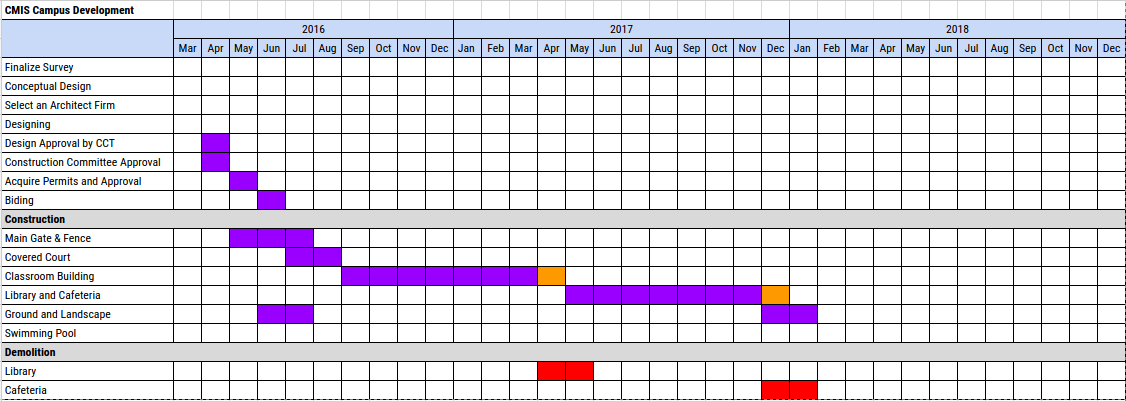
\includegraphics[angle=90, height=\textheight]{profile1}
\caption{Developement Timeline}
\label{figure:devtimeline}
\end{figure}

\subsection{Vision and Mission}

\begin{figure}
\centering

\includegraphics[width=\textwidth]{profile2}
\caption{CMIS Vision and Mission Logo}
\label{figure:visionlogo}
\end{figure}

As a standards-based American curricular school, CMIS offers a challenging educational experience, rooted in Christian values, which helps develop students into global citizens; as reflected in the CMIS vision, mission statement, and learner outcomes.

\minor{CMIS Vision}
To provide educational excellence in a caring community, that respects and celebrates diversity.

\minor{CMIS Mission}
To develop learners who can pursue personal and academic goals, based on educational excellence and strong moral foundations. To equip students for lives of learning and positive contributions locally and globally.

\minor{Student Learner Outcomes}
Courageous learners who:
\begin{itemize}
\item Embody a work ethic that values learning and academic integrity
\item Pursue personal growth as adaptive, independent learners
\item Exhibit thinking that is open minded, creative, and takes risks
\item Utilize resources and technology to effectively support learning and work
\end{itemize}

Responsible global citizens who:
\begin{itemize}
\item Understand Christian virtues and positive student character
\item Demonstrate integrity through consistent respect for people of all faiths
\item Build cultural awareness and an appreciation for diversity
\item Serve as responsible, proactive members of the global community
\end{itemize}

\minor{Student Characteristics}

Excellence in academics and ability to form successful relationships in a multi-cultural Environment.

\minor{School Identity}
 
Developing academic excellence within a multicultural environment committed to Christian Values.

\minor{Religious Affiliation}

CMIS is a school with a clear Christian ethos.  Founded as part of the Church of Christ in Thailand, the national Protestant church, the operation of the school and all relationships within the school community are based upon Christian principles and beliefs with religious services and public prayers offered in the Christian tradition.  Within this spirit, CMIS encourages students to learn about God’s love and the Christian faith so they can make their own personal and intelligent response to it.  CMIS also warmly welcomes students and staff from differing religious backgrounds, cultures, and beliefs.


\minor{So what...}

The market for CMIS is dependent upon tourism and foreign business opportunities in Chiang Mai.  Changes in the economy, political environment, or immigration policies could potentially impact enrollment at CMIS.  Chiang Mai is a popular tourist destination and a pleasant place to live.  At present, the school is experiencing optimal enrollment and a favorable political and social climate.  Our caring community and adherence to Christian values makes us distinct among the other international schools in Chiang Mai.  Our school administrators remain sharply focused on our school mission and vision, while they implement decisions aimed at achieving our Student Learner Outcomes.  CMIS has implemented a development plan to modernize the facility and to accommodate the needs of our growing school community.  

\begin{figure}
\centering
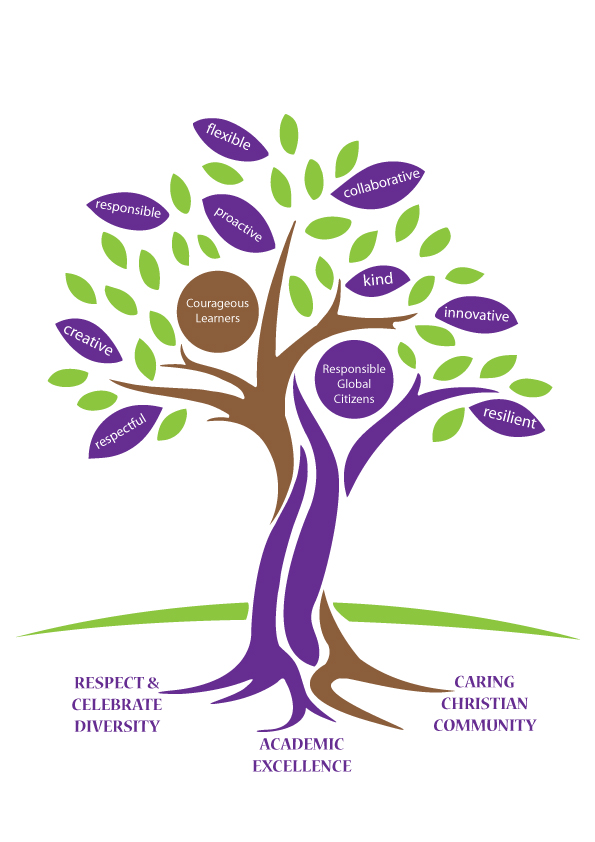
\includegraphics[width=\textwidth]{profile3}
\caption{Tree Logo}
\label{figure:treelogo}
\end{figure}


\tcbsection{Enrollment Patterns}

\minor{Enrollment 2012 - 2016}

Overall student enrollment has increased incrementally by 10 to 20 students per year over the past five academic years.  More than half of the increase came through filling existing vacancies in the Elementary School.  While the Elementary grew at an average rate of 6\% per year, total school enrollment increased by only 2\% per year.  Prior to 2012, Grade 6 was classified as Elementary, whereas from 2013 to present, Grade 6 is classified as Middle School.  Despite the categorical change, Middle School enrollment actually declined slightly throughout the reporting period.  In the 2016-2017 academic year, total school enrollment surpassed 500 for the first time in history.  

As with any international school, CMIS has a small percentage of students who withdraw each year. The resultant vacancies are offset by the enrollment of new students each year.  The balance of enrollment changes each year by accounting for the *previous year’s graduating seniors, adding new and returning students, and subtracting withdrawals.  That annual change is represented in table \ref{table:enrollmentchanges}.



\begin{table}[h]
\caption{CMIS Enrollment Changes}
\label{table:enrollmentchanges}
\begin{tabu} to \textwidth {|X|X|X|X|X|}
\hline
 &
New/Returning*
 Students &
Graduation &
Withdrawals &
Net Increase \\
\hline
2012-2013 &
127 &
36 &
44 &
47 \\
\hline
2013-2014 &
106 &
39 &
59 &
8 \\
\hline
2014-2015 &
120 &
41 &
45 &
34 \\
\hline
2015-2016 &
113 &
38 &
65 &
10 \\
\hline
2016-2017 &
96 &
38 &
-- & 
pending \\
\hline
\end{tabu}
\end{table}

*Returning refers to students who previously attended CMIS, but who had withdrawn for at least one semester.  Continuing students are those who continue their enrollment at CMIS from one year to the next, without interruption.  

In the 2016-2017 academic year, the total number of Continuing vs. New and Returning* students by division is presented in table \ref{table:continuingvsnew}.

\begin{table}[h]
\caption{Continuing vs. New and Returning}
\label{table:continuingvsnew}
\begin{tabu}{|X[2]|X|X|X|}
\hline
&
Continuing&
New/Returning&
Total\\
\hline
Elementary (PK - Gr. 5)&
168 (73\%)&
61 (27\%)&
229\\
\hline
Middle School (Gr. 6 - 8)&
88 (81\%)&
20 (19\%)&
108\\
\hline
High School (Gr. 9 - 12)&
151 (90\%)&
16 (10\%)&
167\\
\hline
TOTAL&
407 (80\%)&
97 (19\%)&
504\\
\hline
\end{tabu}
\end{table}

\minor{So what...}

CMIS replaces approximately 10\% to 20\% of its student body annually.  Sustained, incremental growth has brought us very close to the point of maximum capacity.  However, we have no particular data relating to the reasons people withdraw from CMIS; whether they are satisfied with their CMIS experience, or where they choose to study next.  Because this type of information is available through the Withdrawal Form and the issuing of a School Leaving Certificate, we should be able to obtain meaningful feedback from those who withdraw.  This presents us with an opportunity to survey our withdrawing families and reflect on any trends that might affect our overall enrollment status in the future. 
\tcbsection{Student Diversity}

\minor{Enrollment by Nationality 2015-2016/2016-2017}

The CMIS student body represents a diverse international community, with students from over 30 different countries (see figure \ref{figure:studentdiversity}). The largest single group are those who have dual passport status or parents from two different countries.  Many factors are taken into consideration when selecting our CMIS students.  Age, gender, and nationality are certainly among them.  However, academic potential, the ability to follow instructions, personal maturity, social skills, and overall potential to succeed are of greater importance.  Regardless of \href{https://docs.google.com/spreadsheets/d/15wjkZ9Yy__KpVuhKlawJuoMAAlCE6FMBsOJMKjXacYA/edit?ts=579eee90#gid=0}{nationality} or ethnic identity, all successful applicants must be qualified personally, socially, and academically.  

We give priority enrollment to qualified applicants from the Western world.  There are no restrictions placed on our dual citizens or those coming from Western countries, such as the United States, Canada, the UK, Australia, New Zealand, and English-speaking countries in Europe or Asia.  We do not make exceptions for our missionary or diplomatic communities, but we do reserve spaces for them and give them priority for acceptance, if qualified.  

In the 2016-2017 academic year, the percentage of American, Australian, Canadian, Dual, and United Kingdom students is represented in table \ref{table:AmAuNzCaUk}.

\begin{table}[h]
\caption{American, Australian/New Zealander, Canadian, UK, and Dual Citizenship}
\label{table:AmAuNzCaUk}
\begin{tabu}{|X[2]|X|X|}
\hline
American & 117 & 23\% \\
\hline
Australian / New Zealander & 21  & 4\% \\
\hline
Canadian & 8 & 2\% \\
\hline
Dual & 118 & 23\% \\
\hline
United Kingdom & 26 & 5\% \\
\hline
\end{tabu}
\end{table}

Thai, Korean, Chinese, and Japanese applicants are considered on a space-available basis.  Our target goals for each of these populations compared to our current enrollment is represented in table \ref{table:ThChJa}.

\begin{table}
\caption{Thai, Chinese, and Japanese Enrollment}
\label{table:ThChJa}
\begin{tabu}{|X[2]|X|X|X|}
\hline
Nationality &
Target &
Current Number &
Current Percentage \\
\hline
Thai &
25\% &
183 &
36\% \\
\hline
Korean &
20\% &
75 &
15\% \\
\hline
Chinese &
10\% &
24 &
5\% \\
\hline
Japanese &
10\% &
1 &
<1\% \\
\hline
\end{tabu} 
\end{table}

\begin{figure}
\centering
\caption{2016-2017 Student Diversity}
\label{figure:studentdiversity}
\begin{minipage}{0.5\textwidth}
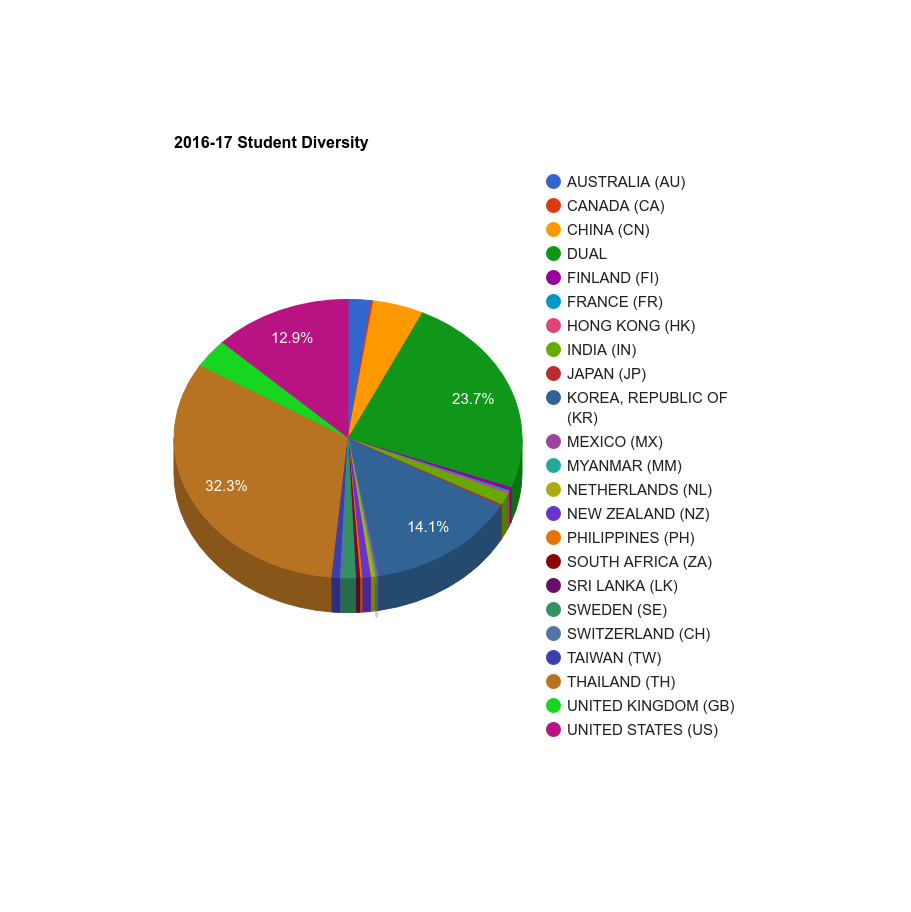
\includegraphics[width=\textwidth]{profile4}
\end{minipage}%
\begin{minipage}{0.5\textwidth}
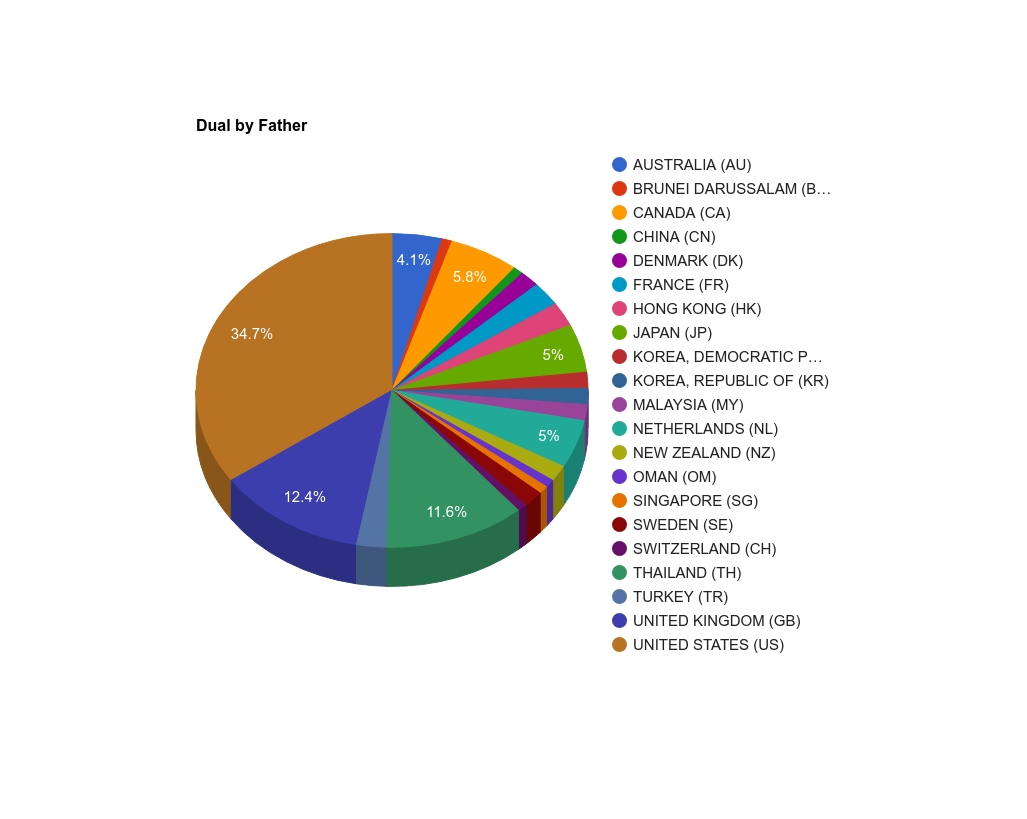
\includegraphics[width=\textwidth]{profile5}
\end{minipage}

\begin{minipage}{0.5\textwidth}
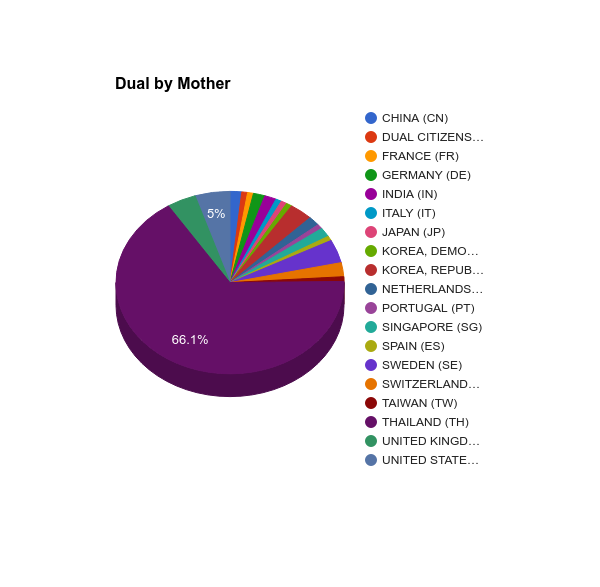
\includegraphics[width=\textwidth]{profile6}
\end{minipage}%
\begin{minipage}{0.5\textwidth}
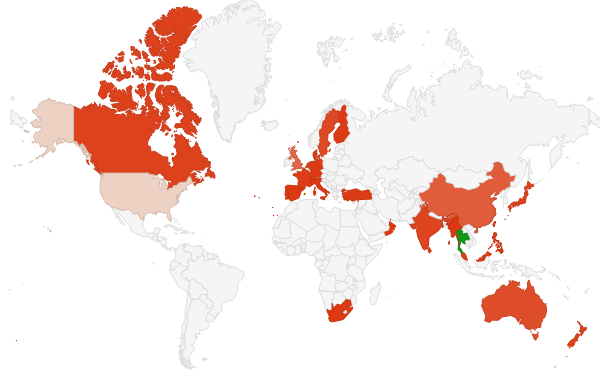
\includegraphics[width=\textwidth]{profile7}
\end{minipage}
\end{figure}

\minor{Teacher/Student Ratios \& Gender Mix}

The ratio of Male (48\%) to Female (52\%) CMIS students remains relatively consistent throughout the student body, with some fluctuation in the Pre-School and Kindergarten grade levels.   With 77 staff in student contact positions (teachers, counselors, IAs) and 504 students, the Teacher / Student ratio is approximately 7:1. See figure \ref{figure:GenderBreakdown} for details.

\begin{figure}
\centering
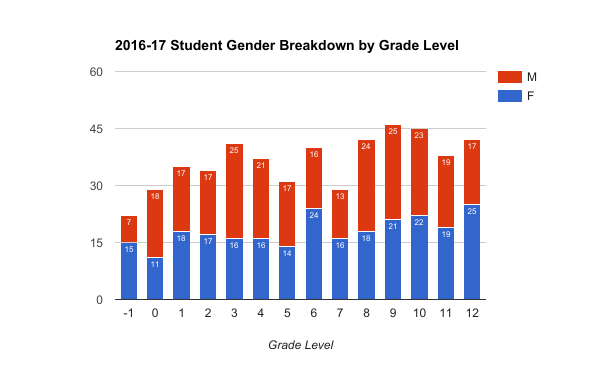
\includegraphics[width=\textwidth]{profile8}
\caption{Gender Breakdown by Grade Level (2016-2017)}
\label{figure:GenderBreakdown}
\end{figure}

\minor{So What...}

CMIS has experienced a period of sustained growth while maintaining ethnic and cultural diversity.  In order to maintain high academic standards in a diverse, English-speaking environment, admissions policies favoring Western applicants will remain in effect.  

\tcbsection{Criteria for Admission of Students}

\subsection{Application Process}

CMIS uses \href{https://cmis.openapply.com/}{Open Apply}, an online application system.  Applicants and enquirers are encouraged to register their interest, schedule an appointment for a meeting with the Admissions Director, and to complete their application electronically.  Applications for first semester enrollment are accepted from January through August.  Elementary and Middle School students may apply for enrollment at any time throughout the semester, provided that appropriate vacancies exist.  High School applications may be considered for enrollment up until the second week of the semester.  Applications received after the cut-off dates will be asked to delay their enrollment until the start of the following semester.  

Rare exceptions are made for High School applicants who are coming from abroad.  In those cases where families move to Thailand in mid-semester, qualified applicants may be accepted into High School in an auditing status.  These students are allowed to attend classes and fully participate in all classroom assignments and activities, although they will not receive credit for the semester course.  

\subsection{Standards for Entry}

CMIS strives to maintain a balanced, harmonious international environment where English is the language of inclusion.  We welcome applications from international students who:
\begin{enumerate}
\item Qualify academically (as determined by school records and standardized entrance assessment results) and
\item Meet the required English-language proficiency expectations for their grade level (as determined by CMIS guidelines).  
\end{enumerate}
CMIS strives to optimize class size to support individualized learning by setting a maximum number of students according to table \ref{table:maxclasssize}.  

\begin{table}
\caption{Maximum Class Size by Level}
\label{table:maxclasssize}
\begin{tabu}{|l|c|}
\hline
Level & Max \\
\hline
Pre-School &  12 \\
\hline
Kindergarten &  15 \\
\hline
Grade 1-2 &	18 \\
\hline
Grade 3-5 &	20 \\
\hline
Grade 6-12 &  25 \\
\hline
\end{tabu}
\end{table}

\minor{Language Proficiency}

Application to CMIS is competitive, and all students must have a minimum level of English language proficiency before they can be considered for enrollment.  The primary conditions for acceptance are academic eligibility, English-language proficiency, and exemplary behavior.  As part of the application process, applicants must submit copies of the current and previous year’s grade reports with teachers' comments, and any relevant standardized test results.  We can accept a limited number of academically qualified non-native English speakers, provided that their English-language proficiency falls within the CMIS guidelines for English Language learners. We can also accept a limited number for students with mild-to-moderate learning disabilities (as determined by previous school records, standardized testing, and Individualized Educational Plans), provided their disability falls within the CMIS guidelines for Learning Support (LS) and there is space available.

\minor{Age Requirements}

CMIS offers a Pre-School program for 4-year-old children who have reached their 4th birthday before the start of school in August.  The age / grade standard is set accordingly throughout elementary; age 5 for entry into Kindergarten, age 6 for grade 1, etc.  All applicants for Pre-School through Gr. 5 must have passed their required birthday by the start of school in August.  Students with birth dates after the start of school in August are classified according to their age on the first day of the academic year thus, any single CMIS grade level may have as much as 11 months of variability in the age of the students.  

For students who apply for entry to Middle School, applicants must have successfully completed the previous academic level and be within the appropriate age range for entry.  The \href{http://cmis.ac.th/admissions}{age/grade level} standard is adhered to as closely as possible.  Transferring into CMIS High School is dependent upon the number of credits on the student's transcript, compared to the CMIS \href{http://cmis.ac.th/programs/high_school}{graduation requirements}.

\minor{Entrance Assessments}

CMIS uses the Early Screening Inventory (ESI) for assessing Pre-School and Kindergarten applicants.  The test is scaled for children 3 years and 6 months old to 6 years 11 months.  Applicants for entry into Grades 1 through 11 are assessed with the WIDA (World-class Instructional Design and Assessment) to determine English-language proficiency.  The WIDA is divided into four grade level clusters:

\begin{itemize}
\item Grades 1 - 2
\item Grades 3 - 5
\item Grades 6 - 8
\item Grades 9 - 12
\end{itemize}


Each form of the WIDA assesses the four language domains of Listening, Speaking, Reading, and Writing.  

\minor{Priority Status}

Although we expect to have annual vacancies at each grade level, we reserve spaces for qualified, priority applicants.  Our Priority Categories are as follows:  
\begin{itemize}
\item Christian Missionary families,
\item Diplomatic / Consular families,
\item NGO / Non-profit organization families,
\item Siblings of current CMIS students,
\item Former CMIS families who are returning from abroad
\item CMIS Staff children, and
\item Fluent English speakers coming from comparable international schools
\end{itemize}

All other applicants are considered on a space-available basis.

In brief, applicants are required to:

\begin{itemize}
\item qualify academically (above average grades in a comparable academic system)
\item demonstrate the English-language proficiency expectations for their grade level
\item fit into a CMIS priority category or add value to our CMIS community
\item succeed academically without ESL or LS, or fit our criteria to qualify for those support programs
\item meet behavioral, emotional and social expectations of the CMIS student body
\end{itemize}

\subsection{Admissions Committee Review Process}

The CMIS Admissions Committee is responsible for making all decisions regarding student applications. The Committee consists of the Admissions Director, School Superintendent, Dean of Students, Elementary Principal, Elementary Counselor, Middle School Counselor, and High School Counselor.    Learning Support Specialists serve as adjunct members of the Committee, and may be asked to comment, provide additional assessment, or recommend further testing.  

In their assessment of an application, the Committee takes the following information into account:

\begin{itemize}
\item applicant's profile
\item previous academic background
\item performance on CMIS entrance assessment
\item English-language ability
\item availability of space at the recommended grade level/support program
\end{itemize}

The Committee determines the applicants’ qualifications for each criteria by:

\begin{itemize}
\item reviewing academic records (minimum of 2 years, as appropriate) and standardized test results
\item conducting entrance assessments
\item reviewing psychologists' assessments or other supporting documentation
\item meetings with the applicant and family
\item reviewing letters of recommendation
\end{itemize}

CMIS uses Open Apply, an online application system.  Applicants and enquirers are encouraged to register their interest, schedule an appointment for a meeting with the Admissions Director, and to complete their application electronically.  

Newly admitted students’ families are given a New Family Survey to help identify areas we need to focus; both in terms of the student application process and advertising. We use this data to refine how we reach our target audience and provide a better experience for our new families.

\tcbsection{School Finance}

CMIS is a privately owned, not-for-profit school.  The \href{https://docs.google.com/document/d/1j2Z1tLgRgfX9CH3dzoYtU_GOhPOVWKPl6iFlvWqd6wM/edit?usp=sharing}{tuition and fee schedule}, as well as the annual operating budget, must be approved annually by the Administrative Advisory Board (AAB). 

\minor{Tuition Rate Categories}

In the 2011-2012 academic year, CMIS instituted a Standard Tuition rate.  All new students from that time onward are classified in the Standard rate category unless the student’s family is eligible for one of the reduced (Discount or Self-Funded Missionary) rate categories.  Those existing CMIS families at that time were automatically grandfathered into the Discount rate category.  This Discount rate also applies to those new expat families who work with NGO’s or Non-profit organizations.  Thus, tuition and fees vary based on each student’s tuition category.  Staff children receive free education as a benefit of their parents’ employment, so Staff children are not required to pay tuition and fees.  

The number of students in each rate category over the past five years is delineated in table \ref{table:tuitionratecat} and figure \ref{figure:numstudentscat}.

\begin{table}[h]
\caption{Tuition Rate Category}
\label{table:tuitionratecat}
\begin{tabu}{|X|X|X|X|X|X|}
\hline
Year &
Standard &
Discount &
Self-Funded &
Staff &
TOTAL \\
\hline
2011-2012 &
45 (10\%) &
230 (52\%) &
128 (29\%) &
38 (9\%) &
441* \\
\hline
2012-2013 &
85 (19\%) &
194 (43\%) &
141 (31\%) &
28 (6\%) &
448* \\
\hline
2013-2014 &
118 (25\%)	 &
174 (37\%) &
136 (29\%) &
43 (9\%) &
471 \\
\hline
2014-2015 &
161 (33\%) &
145 (30\%) &
133 (27\%) &
47 (10\%) &
486 \\
\hline
2015-2016 &
211 (42\%) &
118 (24\%) &
124 (25\%) &
43 (9\%) &
498 \\
\hline
2016-2017 &
250 (49\%) &
92 (18\%) &
118 (23\%) &
47 (9\%) &
507 \\
\hline
\end{tabu}
\end{table}

* Excludes Pre-School.  

\begin{figure}
\centering
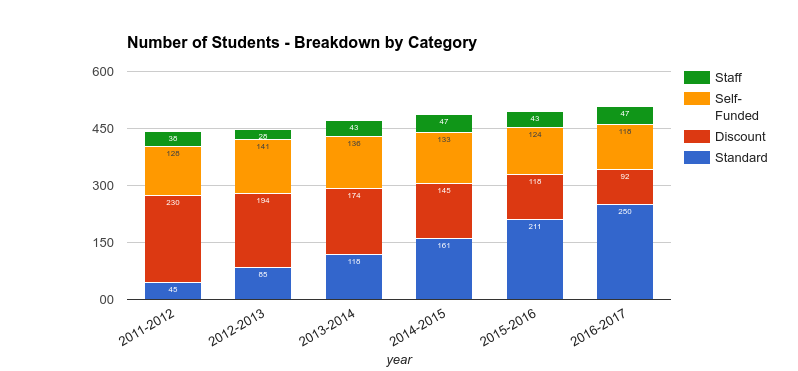
\includegraphics[width=\textwidth]{profile9}
\caption{Number of Students by Category}
\label{figure:numstudentscat}
\end{figure}

Over time, the number and percentage of students in the Standard rate category has increased, while the number and percentage in the Discount rate and Self-Funded Missionary categories has incrementally decreased.  Consequently, the annual income has increased accordingly.  (The number of staff children receiving free tuition has fluctuated with natural changes in our teaching and administrative staff. )  
 
\minor{Income and Expenses}

The graphs below represent the 2016-2017 budget and show anticipated income and categorical projected expenses. See figure \ref{figure:opincex}.  

\begin{figure}
\centering
\begin{minipage}{0.5\textwidth}
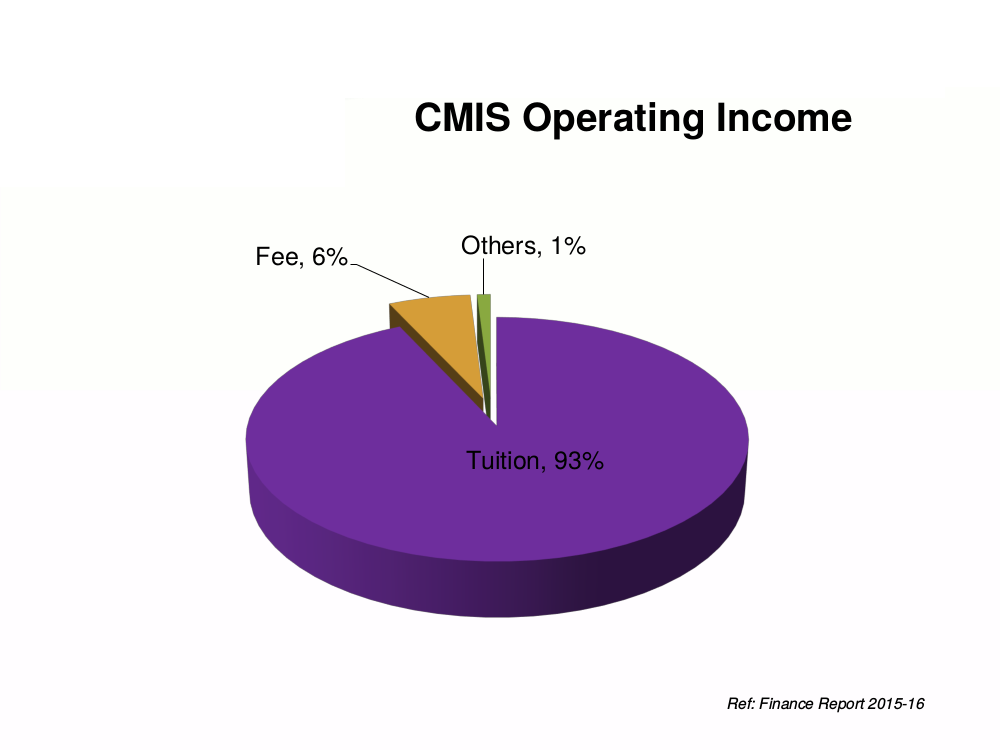
\includegraphics[width=\textwidth]{profile10}
\end{minipage}%
\begin{minipage}{0.5\textwidth}
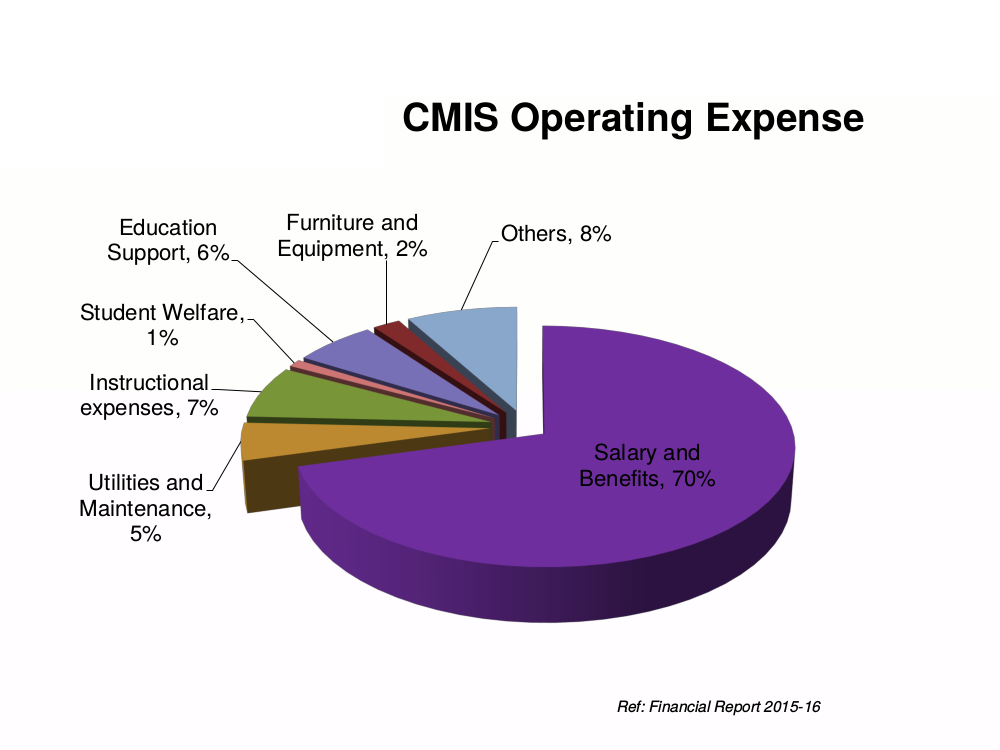
\includegraphics[width=\textwidth]{profile11}
\end{minipage}
\caption{CMIS Operating Income/Expense}
\label{figure:opincex}
\end{figure}

\tcbsection{Faculty and Staff}

\subsection{Administrative Leadership}

CMIS is licensed by the Ministry of Foreign Affairs, owned by the Church of Christ in Thailand (CCT), a national Protestant organization, and operated through a nine-member Board of Directors.  The day-to-day activities of the school are run by a School Management Team (SMT) composed of a Director (Thai), a Superintendent (non-Thai), two Principals (Pre-K - 8 \& High School; non-Thai), a School Manager (Thai), and an Assistant School Manager (Thai). 

\begin{itemize}
\item Director:  Manoonvatana Sirisujin         		director@cmis.ac.th
\item Superintendent:  Ronelda (Nel) Capadona	superintendent@cmis.ac.th
\item ES/MS Principal:  Tyler Stinchcomb	     	elementary@cmis.ac.th
\item HS Principal:  Aaron Willette		   	hsprincipal@cmis.ac.th	
\item Manager:  Patcharin (Nang) Jingkaojai		manager@cmis.ac.th
\item Asst. Manager:  Peay Tananone			assistant\_manager@cmis.ac.th
\end{itemize}

\minor{School Executive Team}

The school executive team (SET) is made up of the director, manager, and superintendent. The SET is responsible for implementing the school vision and mission, and serving as a bridge between the Administrative Advisory Board (AAB) and the school.  They meet weekly to make high level decisions affecting school policies and procedures.  SET members also serve in un-elected positions on the School Board.  

The current school executive team members are:

\begin{itemize}
\item Manoonvatana Sirisujin (CMIS Director) 
\item Patcharin Jingkaojai (CMIS Manager) 
\item Ronelda Capadona (CMIS Superintendent) 
\end{itemize}

\minor{School Management Team}

The school management team (SMT) exists to further implement SET decisions.  The SMT is responsible for the day-to-day, administrative, operation of the school.  The SMT would be involved with issues affecting the school facility, curriculum, and student body. The SMT consists of the SET plus the Assistant Manager, the Elementary/MS Principal, and the High School Principal. 

The current school management team members are:

\begin{itemize}
\item Manoonvatana Sirisujin (CMIS Director) 
\item Patcharin Jingkaojai (CMIS Manager) 
\item Ronelda Capadona (CMIS Superintendent)
\item Tyler Stinchcomb (CMIS Elementary / Middle School Principal)
\item Aaron Willette (CMIS High School Principal)
\item Peay Tananone (Assistant Manager)
\end{itemize}

\minor{Administrative Advisory Board (AAB)}

CMIS is owned by the Foundation of the Church of Christ in Thailand (CCT), and is governed through a Board of Directors comprised of a Board Chair (appointed by CCT); the CMIS School Executive Team; an elected representative from the PTG; an elected representative from the teaching staff; and additional members appointed by the CCT.

The current school board members are: 

\begin{itemize}
\item Rev. Dr. Esther Wakeman (Chair)
\item Rev. Dr. Sharon Bryant (Secretary)
\item Dr. David Filbeck
\item Kathryn McDaniel
\item Manoonvatana Sirisujin (CMIS Director) 
\item Patcharin Jingkaojai (CMIS Manager) 
\item Ronelda Capadona (CMIS Superintendent) 
\item Pascal van Geest (PTG Representative)
\item Brad Schmock (Teacher Representative)
\end{itemize}


The Roles and Responsibilities of the Board (as listed on page 9 of the Student Planner) are included below:

Role of the Board of Directors
\begin{description}
\item [Strategic Planning and Thinking] The Board of Directors develops and maintains the strategic plan for the school, guiding decisions on the organizational level in terms of program, facilities, etc., while keeping in mind the overall vision and mission of the school.
\item [Setting Policy] The Board of Directors oversees the development of policy for school operations. Hiring, evaluating and supporting of the School Leadership Team (Director, Manager and Superintendent) is a key responsibility of the Board. The Board of Directors is not involved in the day-to-day operations of the school, but supports the school leadership in developing the necessary skills and resources to run the school effectively.
\item [Financial Stability] The Board of Directors is responsible for the financial stability of the school and thus sets tuition rates and approves annual budgets.
\item [How Does the Board Govern?] The Board of Directors generally meets once a month from July through June.  Board members should be committed to attending every board meeting, but the board is also understanding of other constraints of members’ time.
\end{description}

\subsection{Professional Staff}

There are currently 65 full-time, \href{http://cmis.ac.th/about/faculty}{professional foreign staff} at CMIS, compared to 57 at the time of our last accreditation (2010-2011).  Increases have come mainly through adding institutional support positions, including Instructional Assistants (IAs) in the lower elementary classrooms, an Elementary Guidance Counselor, an Elementary Learning Support Specialist, and a High School Principal.  An Assistant Manager position was also created to facilitate the implementation of the Building and Facility development plans. See tables \ref{table:totalstaffdept} and \ref{table:totalstaffdeptlevel}.  

\begin{table}[h]
\caption{Total Staff by Department}
\label{table:totalstaffdept}
\begin{tabu}{|X|c|c|}
\hline
&
PK-12 \\
\hline
Admin assistants &
2 \\
\hline
Facilities \& Maintenance &
21 \\
\hline
General &
1 \\
\hline
health/nurse &
2 \\
\hline
Office Staff &
20 \\
\hline
Thai Admin &
3 \\
\hline
Grand Total &
49 \\
\hline
\end{tabu}
\end{table}


\begin{table}[h]
\caption{Total Staff by Department/Level}
\label{table:totalstaffdeptlevel}
\begin{tabu}{|X|X|X|X|X|X|X|X|}
\hline
	 &
ES/MS &
HS &
MS &
MS/HS &
PK-12 &
PK-5 &
Grand Total \\
\hline
Counselors &
&
1 &
1 &
1 &
&
1 &
4 \\
\hline
Foreign Admin &
1 &
1 &
&
&
4 &
&
6 \\
\hline
IA (Thai) &
&
1 &
&
&
&
7 &
8 \\
\hline
learning support & 
&
&
&
&
4 &
&
4 \\
\hline
teachers &
&
15 &
4 &
11 &
&
21 &
51 \\
\hline
Thai teachers &
&
3 &
2 &
1 &
1 &
3 &
10 \\ 
\hline
Grand Total &
1 &
21 &
7 &
13 &
9 &
32 &
83\\
\hline
\end{tabu}
\end{table}

\minor{Staff Diversity}

Our teachers and administrators are well-qualified professionals from 15 different countries, including:  the U.S. (31), Thailand (25), Canada (8), the U.K. (6), the Philippines (2), Myanmar (2), Australia (1), Switzerland (1), the People’s Republic of China (1), France (1), India (1), Mexico (1), the Netherlands (1), Norway (1), and Sweden (1).  More than one-third of our teachers and administrators hold advanced degrees. See figure \ref{figure:adminstaff}.

\begin{figure}
\centering
\begin{minipage}{0.5\textwidth}
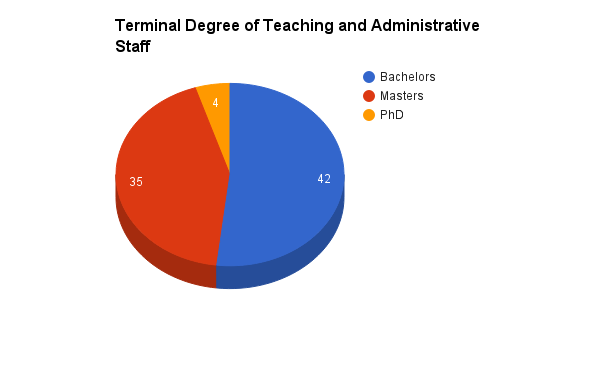
\includegraphics[width=\textwidth]{profile12}
\end{minipage}%
\begin{minipage}{0.5\textwidth}
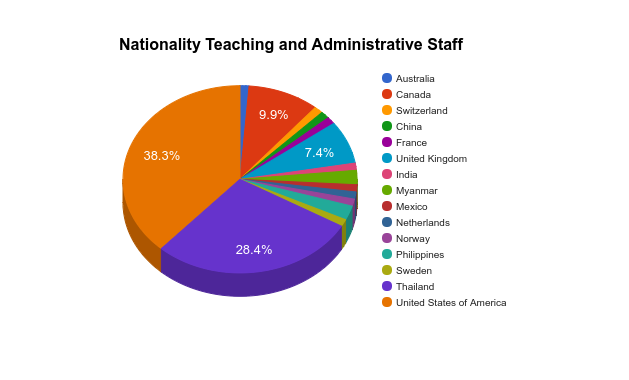
\includegraphics[width=\textwidth]{profile13}
\end{minipage}

\begin{minipage}{0.5\textwidth}
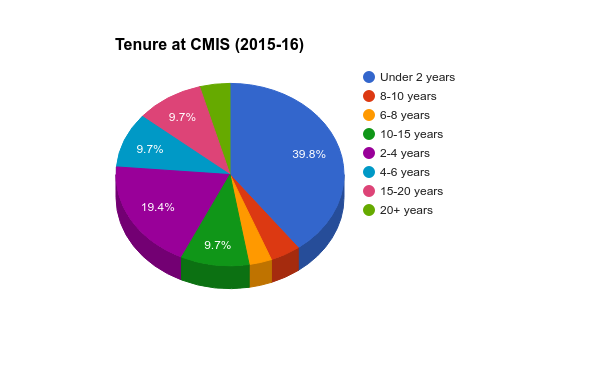
\includegraphics[width=\textwidth]{profile14}
\end{minipage}
\caption{CMIS Administrative Staff}
\label{figure:adminstaff}
\end{figure}

\tcbsection{Staff Professional Development}

CMIS is committed to providing and supporting professional development opportunities for its full-time teachers to improve teaching and student learning. This commitment is grounded in the belief that professional development is a continuous process, one which may be individualized depending on the skills and needs of the teacher; for the purpose of benefiting the teacher, CMIS and its students.  Any professional development opportunity should be related to schoolwide, student learning focus. 

The quality of our Teachers has been identified as the main factor in attracting new students to CMIS.  Recognizing that, CMIS provides teachers and staff with high quality professional development opportunities, both internally and externally.  

CMIS promotes the continued professional development of its teachers in the following ways:

\begin{itemize}
\item On-site scheduled professional development (scheduled during staff meetings and early release days).
\item CMCIS  PD Day - a joint day of collaboration and professional development for schools in the CMCIS, Chiang Mai Circle of International Schools
\item Advanced Placement (AP) Training.  
\item Chiang Mai based Conferences and Seminars. 
\item Online courses and seminars.  
\item Conferences and seminars held in Thailand. 
\item EARCOS Conference.
\item  Out-of-country conferences and seminars. 
\item Sharing the Experience.  Upon the staff member’s return to school, he or she is expected to share with the school what was learned.  Staff members are also required to file a written assessment of the program through the Professional Development Assessment Form that will be made available for other staff to review.
\end{itemize}


\minor{Designated Funding}

In addition to school/department wide professional development, the school provides funding in the amount of 10,000 Baht for each school year (starting in the 2013-14 school year), for each full-time teacher to engage in professional development (PD) opportunities.  PD funds can be accrued up to 5 years. Any (projected) unspent amount will be returned to the general PD fund at the end of the 5-year period or earlier if the teacher leaves CMIS employment. Since 2014, the school has utilized over 1,370,000 baht from the professional development budget.

The professional development (PD) budget may be used toward recertification, workshops, conferences, professional memberships, or position-specific training.  Travel, per diem, accommodation, registration, tuition, and required materials are also eligible for reimbursement, based on established guidelines.  Transportation budgets are limited, and staff are encouraged to look for PD opportunities within the region.  

All professional development funding and leave must be approved by the divisional principal, superintendent, or director.  All applications for professional development are considered carefully based on the following:

\begin{itemize}
\item Location of the event with priority set in the order of Chiang Mai, Thailand, SE Asia, outside of SE Asia, as well as if the course or seminar is offered online.
\item Relevance to the school wide, student learning focus.
\item Benefit to CMIS.
\item Length of time away from school.
\item Budget availability (early application is best for this).
\item Timing of request, advanced notice is preferred.
\item Staff member’s seniority or stated plans to stay at CMIS.
\end{itemize}

\begin{figure}
\centering
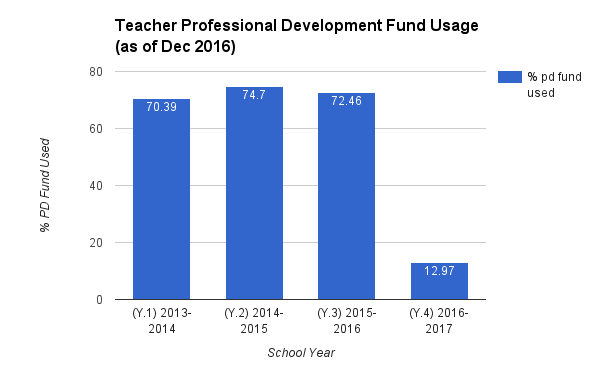
\includegraphics[width=\textwidth]{profile15}
\caption{Teacher Professional Development Fund Usage (as of December 2016)}
\end{figure}

CMIS Teachers and administrators are hired on two-year contracts.  More than half of our foreign staff (59\%) have been in their current positions for four years or less, while 25\% have been here for 10 or more years. 

\tcbsection{Teacher/Administration Communication Team (TACT)}

CMIS employees should have a safe and positive working environment. We understand that when working as a team, misunderstandings or miscommunication may occur.  In an effort to alleviate this, CMIS created the Teacher Administration Communication Team (\href{https://docs.google.com/a/cmis.ac.th/document/d/14nhwcw8xo3i-23Q-WUxo6KJ_c8yFKu-jTdCctt4MFcs/edit?usp=sharing}{TACT}) in 2013. The team is comprised of teacher reps from each division and the school executive team. The team meets regularly to review and address current staff concerns and a \href{https://docs.google.com/a/cmis.ac.th/document/d/1KLB4c5_LkxXzq4vP2EuNhBVPp2q_FT9qy1cBBwaS5JM/edit?usp=sharing}{summary} of the solutions and suggestions are e-mailed out to all staff.

The purpose of the \href{https://docs.google.com/document/d/12ZwL4geAPTDcm-SI6U1fRpXEKxKZ-61q54upcikt6lc/edit}{TACT} is to foster and create the best learning environment possible for our students by improving the overall happiness and satisfaction of faculty. We believe that when we invest in the well being of people, we invest in the long-term success and viability of CMIS.

To this end, the role of TACT is to provide a way for faculty to raise issues, concerns, and questions to the CMIS Executive Team (Director, Superintendent, Business Manager).  CMIS prefers that individuals address issues, concerns, and questions directly to their building administration (the principals of the elementary, middle, and high schools).  There are times, however, when individuals may not feel comfortable in speaking with building administration or leadership; thus TACT can forward these issues on their behalf.

\begin{itemize}
\item we believe in positive intentions, and that all stakeholders share the same vision of the best possible learning environment for CMIS students
\item we believe in openness and transparency in decision making and communications
\item we believe in equity - the fair and impartial treatment of others
\item we believe that praise and recognition produces far better results than criticism or punishment
\item we believe in social sustainability and social responsibility
\end{itemize}

\tcbsection{Parent Teacher Group (PTG)}

Teachers, administrators and parents or guardians of CMIS students are all automatically members of the Parent Teacher Group (PTG). The PTG is the "voice" at CMIS, as it provides a forum for sharing ideas and concerns about the school, and creates opportunities for parents and staff to establish friendships and networks within the CMIS community. The primary objectives of the PTG are:

\begin{itemize}
\item To promote communication between CMIS parents, teachers and administrative staff.
\item To promote and actively support CMIS educational programs, sports, activities and events.
\end{itemize}
 
The PTG achieves this through volunteer work and fundraising.  The PTG welcomes and encourages all parents and teachers to take an active role in the school by attending monthly meetings, and by volunteering time, resources and abilities to make CMIS the best place that it can be for our students.

The PTG serves as a conduit of communication between teachers, administrators, parents, and members of the school community.  

\tcbsection{Non-Academic Activities}

\subsection{Beyond the Classroom}

CMIS offers opportunities for student growth and personal development through Student Life Beyond the Classroom programs and activities.  

\minor{What is Student Life?}

“Student Life” is a common division, department, or office found on university and college campuses across the United States of America.  These divisions can be designed to meet a broad range of student needs/concerns, but they all have the basic goal of helping students get the most out of their experiences at school by supporting student opportunities away from the classroom.  At CMIS, student life is defined as the beyond the classroom opportunities which align with the CMIS Mission Statement and allow for personal, social, spiritual, intellectual, artistic, and physical growth.

\minor{Faith and Service}

CMIS encourages faith and service outside the classroom by allowing students to pursue their unique interests both on and off campus. The school invites students to initiate their own faith-based groups, and it encourages students to use school facilities to hold meetings and events.  In 2015, CMIS created a position of  a Student Spiritual Advisor.  The advisor is a faithful role model and spiritual guide for not only our Christian students, but all students. The advisor is there to listen to the students, hear where they are coming from, give them confidence and support, share advice if asked, and help them navigate life as a person of faith. The Spiritual Advisor also facilitates the CMIS Community Service Program that supports high school students in completing 60 hours of \href{http://cmis.ac.th/programs/community_service}{community service} before graduation. CMIS defines community service as making a difference through actions of caring for others, either in the school or in the community.  It includes direct service, indirect service, and advocacy. CMIS high school students have put in more than 16,500 community service hours since the 2013-14 academic year.

\minor{Clubs and Activities}

CMIS offers a variety of activities, clubs and student organizations for students after school.  These opportunities allow students to pursue passions, explore new interests, and gain valuable leadership experience while working alongside an adult group leader/adviser.  To see a full list of up-to-date offerings for the elementary, middle, and high school levels, visit the below links.
\href{http://blogs.cmis.ac.th/eagles/clubs-activities/es/}{Elementary clubs and activities}
\href{http://blogs.cmis.ac.th/eagles/clubs-activities/ms-hs/}{MS and HS clubs and activities}

\minor{The Arts}

In addition to being committed to offering a curriculum that values visual arts, music, drama, and dance, CMIS strives to provide opportunities outside of the classroom for students to be able to further their own understanding of, appreciation for, and talents in the visual and performing arts.

\minor{Athletics}

CMIS offers a variety of athletic programs at various levels of competition to students.  The CMIS Athletic Department recognizes extra-curricular opportunities as a way to stimulate intellectual, emotional, social, and physical growth outside of the classroom walls.  Our programs encourage a team-building approach that emphasizes leadership, commitment, excellence, and communication.  Our goal is to foster a positive student-athlete culture on campus through collaboration with students, parents, faculty, staff, and administration to ensure student-athletes remain academically focused at the same time that they are engaged in a dynamic, challenging, and safe learning environment.

\minor{Student Government}

CMIS Administration encourages growth and development of its students by allowing the establishment and operation of various student activities. Student Council (StuCo), as one of the most important activities, acts as a planning and representational body on behalf of certain student interests.

CMIS StuCo is a representative structure for all the students in Middle School \& High School.  It provides students with the opportunity to become involved in the affairs of the school, working in partnership with school management, staff, community, and parents.  It is intended to work for the benefit of the school and its students. 
 
The \href{https://docs.google.com/a/cmis.ac.th/spreadsheets/d/1Dew5VG0EEek2lvCfLnK5dQa1G-KFTZV3qzR0FFJW1hA/edit?usp=sharing}{CMIS Student Council Organizational Chart}, the \href{https://docs.google.com/document/d/1eQY8B1nPq12prl7nvG42gDSqu9BSYTu-HvTZ22xnCjE/edit?usp=sharing}{CMIS Student Council (StuCo) Structure and Roles}, as well as the \href{https://docs.google.com/document/d/1jyWCNvdDBbUYXTOtACMD4BrgnmwtGNdOdigtEbqqMuM/edit?usp=sharing}{StuCo HS \& MS Activities} are further detailed in the attached links.  

\subsection{Student Health}

CMIS has a registered Thai Nurse on staff at all times, as well as a Foreign Health Officer, who coordinate CMIS programs and activities related to general health and safety; including health and fitness, immunizations, environmental quality, sanitation practices, vector control, evacuation drills, and cafeteria coordination.  The CMIS Health Office’s areas of responsibility include:

\minor{Measures of overall student Health \& Fitness }
\begin{itemize}
\item Eye examination (including color blind test)
\item Weight and Height measurements and calculation of BMI. 
\item Students in G5-G8 also have a scoliosis examination. 
\end{itemize}


\minor{Reporting Criteria}
\begin{itemize}
\item All results of student health assessments are recorded in the Health Section of Powerschool. Results are shared with Parents via e-mail with recommendations for treatment.
\item In addition, parents complete a Health Form at the beginning of each year detailing any illness or allergies students have. Vaccination records are also collected. Information is kept in paper form in Health Office and also in Openapply and Powerschool.
\item Visits to the Health Office are recorded daily. Results are collated onto a spreadsheet which details how many students from each grade have been in the Health Office that month. The reasons for attending the Health Office are also collated, helping to look for trends. The spreadsheet is shared with the SET monthly.
\item All teachers can access emergency information regarding students with allergies via Powerschool. Information is also sent to specific teachers via email.
\end{itemize}


\minor{\href{https://sites.google.com/a/cmis.ac.th/cmis-health-office/}{Health Services}}
\begin{itemize}
\item Individualized healthcare plans are completed for all Students with medical conditions and stored in their file in the Health Office.  
\item Medication administration is recorded for each student who require it, and records are stored in the Health Office.
\item Health Alerts for students with allergies or serious medical conditions are posted in Staff room and cafeteria with details of their allergy or illness and instructions on how to manage.
\end{itemize}


\minor{Environmental Quality and Monitoring}
\begin{itemize}
\item Drinking water is tested monthly and results are recorded on a spreadsheet which is shared with teachers and parents.
\item Governmental health representatives come to test the cafeteria food annually, if possible.  
\item Accidents are recorded on individual Accident Forms which are shared with the Superintendent.  Original forms are filed in the Health Office for review and trend analysis.  
\item The Health Office and the Athletic Department monitor the pollution levels throughout the day by checking the Air Quality Index (AQI) as posted by the Pollution Control Department of the Thai Government. (\href{http://aqmthai.com/}{http://aqmthai.com/}).  Precautions are recommended according to the \href{https://docs.google.com/document/d/1RLrOBWjj_4ohMofL5RUIaWWwP66qTJ2NFEl_qY5U5Vw/edit?usp=sharing}{established guidelines}.  
\end{itemize}

\minor{Cafeteria Coordination}
\begin{itemize}
\item An \href{https://docs.google.com/spreadsheets/d/1Z2Wcw-UM1njZZ51OefDeCqH8mDTJvaefXS_WJbK4Z20/edit#gid=1328983646}{annual Cafeteria survey} is given to students in G2-G12. 
\item The school reacts to these results and works with the cafeteria to try to improve the cafeteria (e.g., moving snacks outside, introducing a 1-month rolling menu, adding additional menu options, etc.)
\item The cafeteria aims to make food as healthy and tasty as possible using quality ingredients without preservatives or additives. All the bread, tortillas, lasagna, buns, tacos and sauces are homemade from scratch and all vegetables are organic or pesticide free (from Monkey farm or the King’s projects)
\end{itemize}

\subsection{Student Discipline}
Student Planners contain the student handbook; which outlines school rules, regulations, procedures, and policy; as well as student rights and responsibilities.  Students are given a Student Planner at the beginning of each school year.  The information is also available on the school website for easy access and reference.  Consequences for major violations of school rules and policies are tiered and articulated in the handbooks. 

CMIS faculty and administration annually review and update student and teacher handbooks as well as revise and add policy where needed. 

The majority of CMIS students display positive and respectful behavior. When there are transgressions of good conduct, consequences follow a response to intervention ( RTI) approach and are addressed accordingly:

\begin{enumerate}
\item Minor offenses are redirected through classroom management strategies 
\item Moderate offenses are managed through teacher intervention and communicated to the parent
\item Repeated offenses are referred to the Student Success Team (teacher, counselor, student service coordinator, and principal) and an Intervention Plan is created with the parents. 
\item Severe offenses that cause serious physical or emotional injury to self or others are referred to the Administrative Team (Principals and Superintendent). 
\end{enumerate}

Generally, suspension is only applied when other interventions have failed or when a sudden, serious offense occurs. A conference with the student’s parents is required prior to re-admittance to classes after either an in-school or out-of-school suspension. 

The most common infractions during 2015-2016 school year were dress code violations in the MS/HS.  Major and minor infractions are kept in Powerschool discipline logs. Out-of-school suspensions are rare at CMIS.

\tcbsection{Academic Performance Data}

\subsection{Developmental Reading Assessments (DRAs)}

CMIS places strong emphasis on the importance of reading.  Elementary students are required to read at least 20 minutes daily, and CMIS parents are asked to verify their child’s efforts.  Even Kindergarten students, who are just learning to read, are given opportunities to read \href{https://www.raz-kids.com/}{Raz Kids}, an online reading program, and to check out library books regularly.  All elementary students receive an individual Raz-Kids log on, which can be accessed both at school and at home.  Elementary students have one designated class in the Computer classroom each week in order for their Homeroom teacher to observe their use of Raz-Kids.  They also have a Library class as one of their Specials, in which they are given guidance and direction in finding and checking out appropriate level reading materials.  

To monitor elementary students’ reading ability, \href{https://drive.google.com/open?id=0ByVFfrm0zfolV29lcmM1WXVQOXc}{Developmental Reading Assessments (DRAs)} are conducted twice annually.  The DRA is a standardized reading test used to determine a student’s instructional level in reading. The DRA is administered individually to students by the homeroom teachers. Students read one or more selections and then retell what they have read to the examiner. Those students who are identified to be reading below their grade level are targeted for reading support in the classroom. 

In general, the percentage of students who are reading “on” grade level gets smaller in each successive grade level, which is common as the difficulty level for each selection increases as the student progresses to the next level. While the percentage of students in the “Above” category tends to increase at each grade level, the percentage of those who fall “Below” the grade level standard fluctuates as well. This broad spectrum of reading ability requires CMIS teachers to differentiate the reading instruction in order to help all students meet the required Student Learner Outcomes.  

 
\begin{figure}
\centering
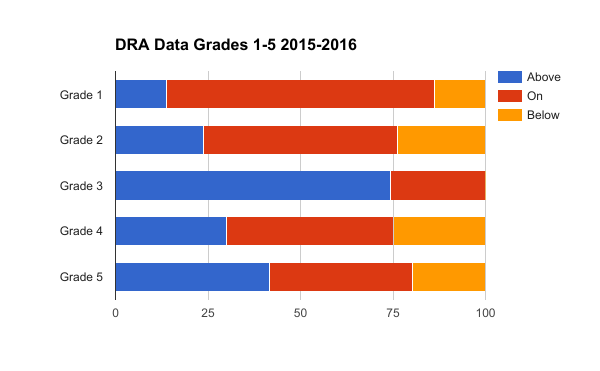
\includegraphics[width=\textwidth]{profile16}
\caption{DRA Data Grades 1, 2, 4, and 5 2015-2016}
\end{figure}

\subsection{International Schools’ Assessment (ISA)}

Historically, CMIS has given the \href{https://drive.google.com/drive/u/0/folders/0B71_pYxcTLo-anRvTzA5NDBGUW8}{ACER ISA} (International Schools’ Assessment) test to students in grades 3, 5, and 7.  Data from these tests show CMIS students performing as well as or better than both “All Students” taking the ACER ISA and students categorized in “comparable schools” with the same percentage of students from an English-speaking background.  Comparisons were done using the Student’s t-test. 

\begin{table}
\caption{English Speaking Background}
\label{table:10}
\begin{tabu}{|c|X|c|}
\hline
Academic Year &
CMIS \% of English Background Speakers &
ISA Group \\
\hline
2011-2012  &
41 to 55\% &
3 \\
\hline
2012-2013  &
26 to 40\% &
2 \\
\hline
2013-2014  &
26 to 40\% &
2 \\
\hline
2014-2015  &
41 to 55\% &
3 \\
\hline
2015-2016  &
36 to 55\% &
3 \\
\hline
\end{tabu}
\end{table}

Based on our reported percentage of students from an English-speaking background, CMIS is categorized differently by ISA each year.  For example, in the 2011-1012 academic year, CMIS was initially categorized in ISA Group 3.  However, from 2012 to 2014, CMIS demographics shifted to 26 to 40\% of students from an English speaking background, placing us in ISA Group 2.  In the 2014-2015 academic year, the percentage of CMIS English background students increased to 41 to 55\%, shifting us into ISA Group 3.  In the 2015-2016 academic year, while the percentage of CMIS English background students fluctuated from 36 to 55\%, we remained within the range of ISA Group 3.  Thus, a year by year comparison with comparable schools is hard to make and interpret.  For an individual student taking the test in Grades 3, 5, and 7, a comparison is made to students in schools with different demographics.  Because the ranking of an individual student changes with the respective ISA Group, it is impossible to see relative progress over time.  

During the Data Wise initiative 2015-2016, a study of the ISA data identified the need for students to further develop their Expository/Argumentative Writing skills.  A \href{https://drive.google.com/drive/folders/0ByVFfrm0zfolLU9Vb0ZBeF9uZjQ}{school wide writing assessment} was given to further confirm this need, and an action plan was created to scaffold the students that needed extra attention with this particular skill. Tools such as graphic organizers were created and placed in classrooms.  We also created a \href{https://docs.google.com/document/d/1JvVcmrIylkSYJeT4vgbyrqQTfZuJW-Iu6GB6jNCreIU/edit?ts=58a5129f}{common assessment rubric for English Language Arts (ELA) 9-12}.  Using Acer ISA in Datawise was challenging for the following reasons: 
\begin{itemize}
\item the category of schools CMIS falls into changes based on the percentage of students from an English-speaking background, thus making a year by year comparison difficult.
\item The Standards addressed in the ISA tests were not the same standards used at CMIS.
\item Students are tested in grades 3, 5, and 7.  The long time interval between tests does not support modifying instruction to fit student needs.
\end{itemize}

\begin{table}
\caption{Average ISA Test Results (Grade 3), 2011-2016}
\label{table:11}
\begin{tabu}{|X[2]|X|X|X|X|X|}
\hline
  &
2011-12 &
2012-13 &
2013-14 &
2014-15 &
2015-16 \\
\hline
\multicolumn{6}{|l|}{Mathematical Literacy} \\
\hline
CMIS &
315 &
365 &
334 &
344 &
327 \\
\hline
All Schools  &
310 &
334 &
308 &
330 &
327 \\
\hline
\multicolumn{6}{|l|}{Reading} \\
\hline
CMIS  &
263 &
293 &
292 &
323 &
319 \\
\hline
All Schools  &
254 &
255 &
266 &
291 &
257 \\
\hline
\multicolumn{6}{|l|}{Writing A} \\
\hline
CMIS  &
381 &
374 &
409 &
367 &
377 \\
\hline
All Schools  &
375 &
364 &
378 &
378 &
363 \\
\hline
\multicolumn{6}{|l|}{Writing B}\\
\hline
CMIS  &
405 &
396 &
430 &
407 &
389 \\
\hline
All Schools  &
392 &
395 &
409 &
413 &
391 \\
\hline
\end{tabu}
\end{table}

\begin{figure}
\centering
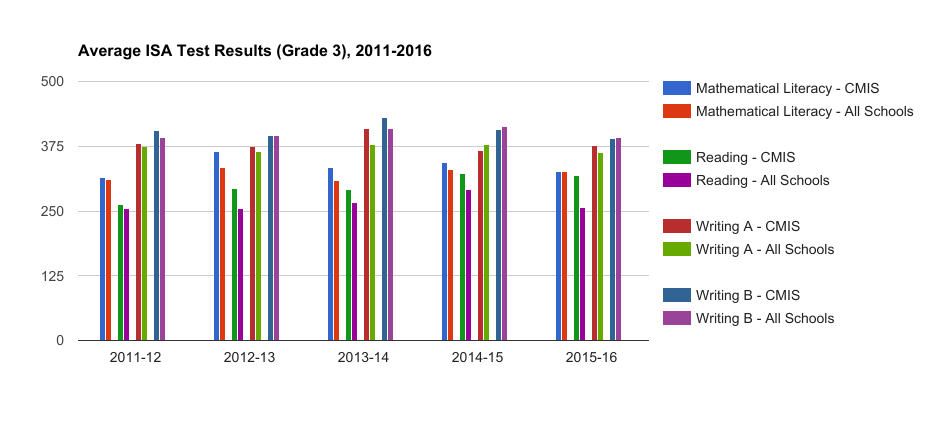
\includegraphics[width=\textwidth]{profile17}
\caption{Average ISA Test Results (Grade 3) 2011-2016}
\end{figure}

\begin{figure}
\centering
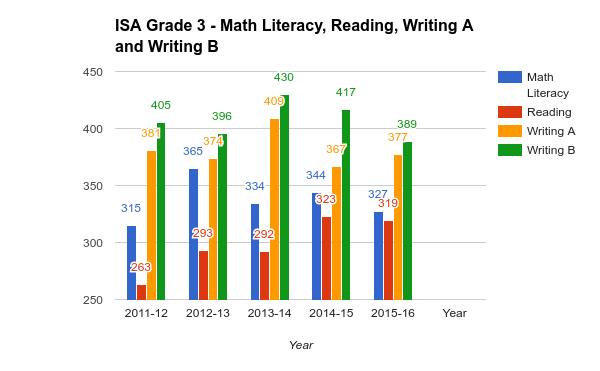
\includegraphics[width=\textwidth]{profile18}
\caption{ISA Grade 3 - Math Literacy, Reading, Writing A and Writing B}
\end{figure}

\begin{table}
\caption{Average ISA Test Results (Grade 5), 2011-2016}
\label{table:12}
\begin{tabu}{|X[2]|X|X|X|X|X|}
\hline
&
2011-12  &
2012-13 &
2013-14 &
2014-15 &
2015-16 \\
\hline
\multicolumn{6}{|l|}{Mathematical Literacy} \\
\hline
CMIS  &
444 &
486 &
471 &
458 &
449 \\
\hline
All Schools  &
417 &
424 &
432 &
444 &
427 \\
\hline
\multicolumn{6}{|l|}{Reading} \\
\hline
CMIS  &
432 &
412 &
385 &
460 &
441 \\
\hline
All Schools  &
381 &
357 &
362 &
396 &
361 \\
\hline
\multicolumn{6}{|l|}{Writing A} \\
\hline
CMIS  &
494 &
486 &
472 &
475 &
486 \\
\hline
All Schools  &
455 &
451 &
461 &
460 &
455 \\
\hline
\multicolumn{6}{|l|}{Writing B} \\
\hline
CMIS  &
487 &
498 &
484 &
487 &
513 \\
\hline
All Schools  &
465 &
467 &
487 &
482 &
467 \\
\hline
\end{tabu}
\end{table}

\begin{figure}
\centering
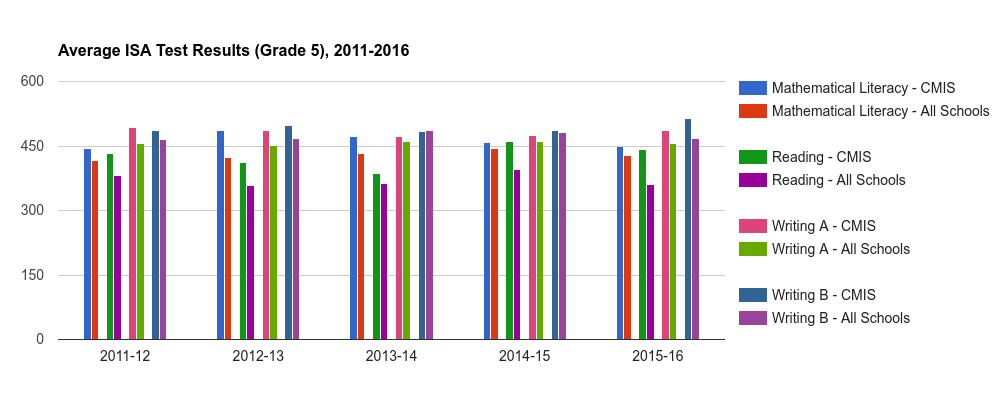
\includegraphics[width=\textwidth]{profile19}
\caption{Average ISA Test Results (Grade 5), 2011-2016}
\end{figure}

\begin{figure}
\centering
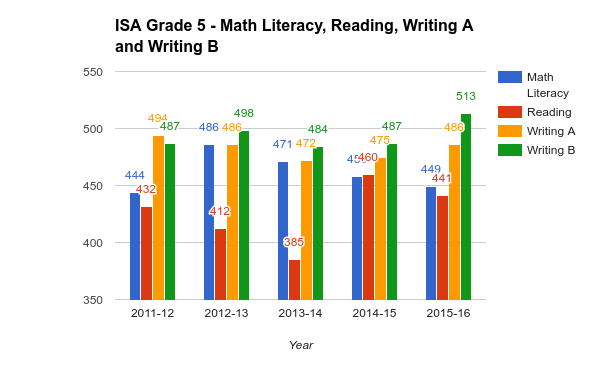
\includegraphics[width=\textwidth]{profile20}
\caption{ISA Grade 5 - Math Literacy, Reading, Writing A and Writing B}
\end{figure}

\begin{table}
\caption{Average ISA Test Results (Grade 7), 2011-2016}
\label{table:11}
\begin{tabu}{|X[2]|X|X|X|X|X|}
\hline
  &
2011-12 &
2012-13 &
2013-14 &
2014-15 &
2015-16 \\
\hline
\multicolumn{6}{|l|}{Mathematical Literacy} \\
\hline
CMIS  &
534 &
582 &
559 &
545 &
526 \\
\hline
All Schools  &
486 &
504 &
521 &
512 &
507 \\
\hline
\multicolumn{6}{|l|}{Reading} \\
\hline
CMIS  &
526 &
515 &
500 &
504 &
495 \\
\hline
All Schools  &
454 &
447 &
451 &
448 &
457 \\
\hline
\multicolumn{6}{|l|}{Writing A} \\
\hline
CMIS  &
553 &
550 &
546 &
569 &
526 \\
\hline
All Schools  &
512 &
511 &
525 &
526 &
517 \\
\hline
\multicolumn{6}{|l|}{Writing B} \\
\hline
CMIS  &
531 &
550 &
528 &
534 &
541 \\
\hline
All Schools  &
518 &
523 &
540 &
533 &
525 \\
\hline
\end{tabu}
\end{table}

\begin{figure}
\centering
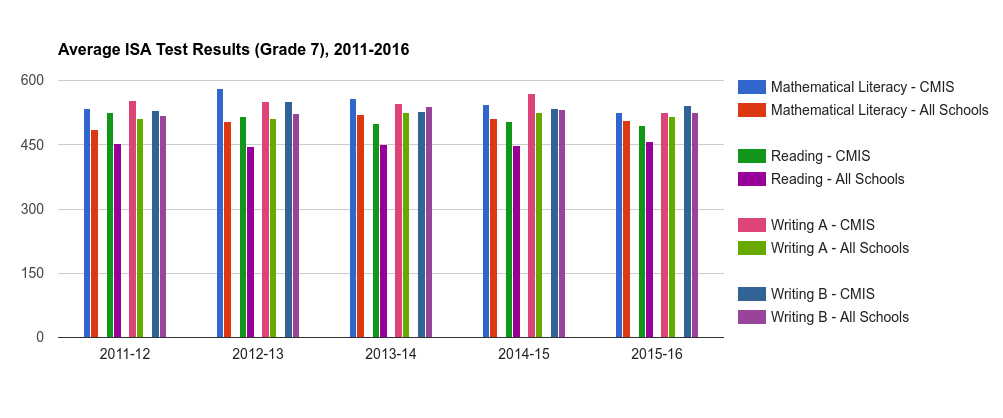
\includegraphics[width=\textwidth]{profile21}
\caption{Average ISA Test Results (Grade 7), 2011-2016}
\end{figure}

\begin{figure}
\centering
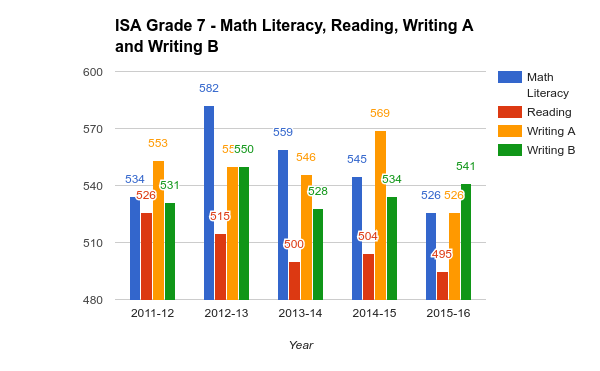
\includegraphics[width=\textwidth]{profile22}
\caption{ISA Grade 7 - Math Literacy, Reading, Writing A and Writing B}
\end{figure}

\subsection{Northwest Evaluation Association (NWEA) Measures of Academic Progress (MAP)}

CMIS has re-adopted the NWEA MAP (Measures of Academic Progress) test, starting in January 2017. (It was previously used in the 2011-2012 academic year.)  School Administrators anticipate that MAP will provide more useful data, as each student in Gr. 2-10 will be tested twice annually.  MAP tests are based on the Common Core objectives for each respective grade level.  

\subsection{PSAT 8/9}

All students in grades 8 and 9 take the Practice Scholastic Aptitude Test 8/9 (PSAT 8/9) in October, in accordance with the dates set by the College Board. According to the global data compared with the random selection of PSAT results from around the world, the majority of CMIS students perform better than the mean. In general CMIS students excel on these tests.   PSAT test-takers receive a copy of their results and are asked to use them to help target areas where they need improvement.  

The scores for the\href{https://docs.google.com/a/cmis.ac.th/spreadsheets/d/1OVMnw4x1eUg-QByMt2J2IZJkovZGys_8uoj1SKSM2As/edit?usp=sharing}{ first two years for the PSAT 8/9 (2015-17)} are shown below as compared to a sample of n=1,000 for the PSAT 8/9.  Center lines show the medians; box limits indicate the 25th and 75th percentiles as determined by R software; whiskers extend 1.5 times the interquartile range from the 25th and 75th percentiles, outliers are represented by dots; crosses represent sample means. Blue indicates grade 8, yellow is grade 9, and green represents the combined score of grades 8 and 9.  

With the exception of outliers, almost all CMIS students tested scored above the median score of the sample group.  

\begin{figure}
\centering
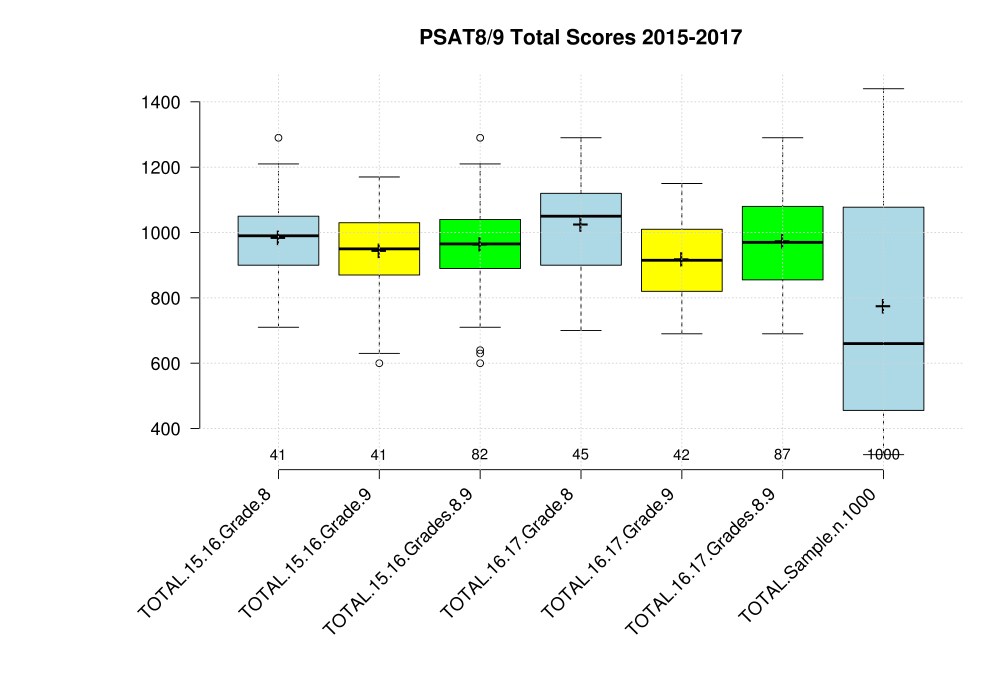
\includegraphics[width=\textwidth]{profile23}
\caption{PSAT8/9 Total Scores 2015-2017}
\end{figure}

\begin{figure}
\centering
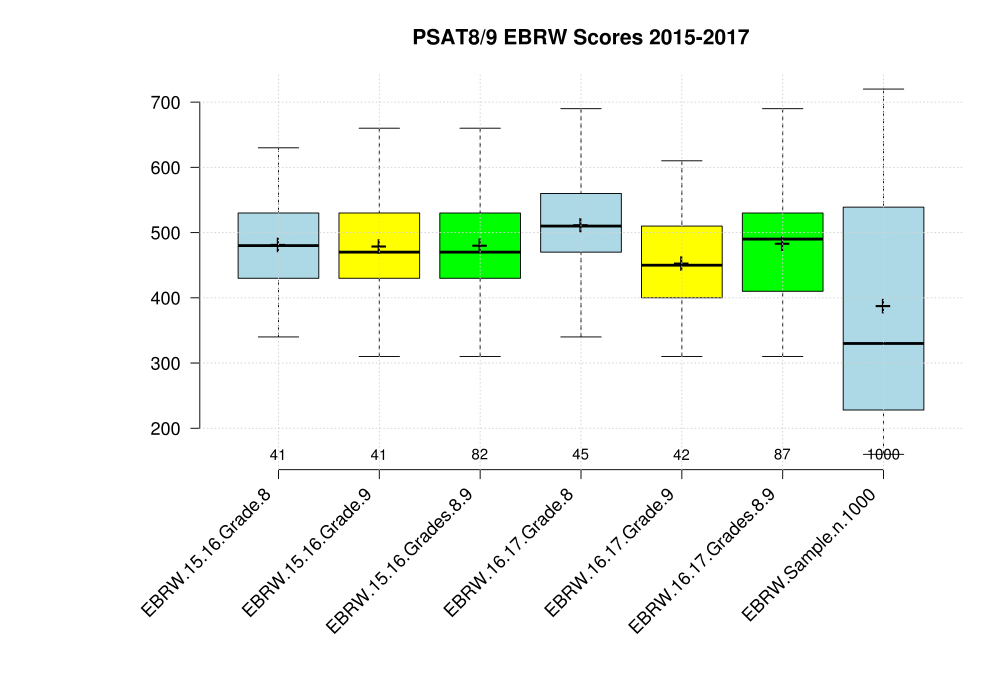
\includegraphics[width=\textwidth]{profile24}
\caption{PSAT8/9 EBRW Scores 2015-2017}
\end{figure}

\begin{figure}
\centering
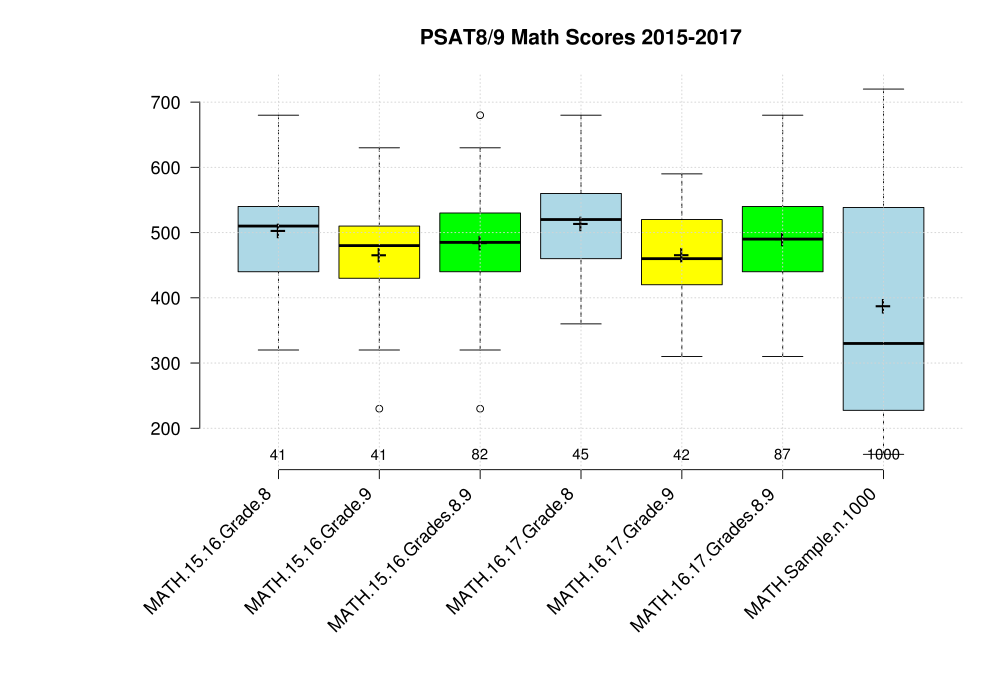
\includegraphics[width=\textwidth]{profile25}
\caption{PSAT8/9 Math Scores 2015-2017}
\end{figure}

\subsection{PSAT/NMSQT}

Students in grades 10 and 11 take the Preliminary Scholastic Aptitude Test\href{https://drive.google.com/drive/folders/0B71\_pYxcTLo-VGNkQlZtTFlIQlE}{ (PSAT) / National Merit Scholarship Qualifying Test (NMSQT)} in October, in accordance with the dates set by the College Board. According to the global data compared with the random selection of PSAT results from around the world, the majority of CMIS students perform better than the mean. In general, CMIS students excel on these tests.  In fact, one of our students was nominated for the National Merit Scholarship Award by scoring in the top 5\% of all PSAT test-takers in 2015.  PSAT test-takers receive a copy of their results to help target areas where they need to improve before taking the SAT exam.  

\minor{\href{https://collegereadiness.collegeboard.org/about/scores/benchmarks}{Benchmark Indicators}}

Score reports use colors to show how students’ section scores relate to the SAT or grade-level benchmark.
\begin{itemize}
\item Green: The section score meets or exceeds the benchmark.
\item Yellow: The section score is within one year’s academic growth of the benchmark.
\item Red: The section score is below the benchmark by more than one year’s academic growth.
\end{itemize}

\minor{SAT College and Career Readiness Benchmarks}

Evidence-Based Reading and Writing: 480

Math: 530

SAT Section Score Ranges

200-800 Point Scale
 
\begin{tabular}{|l|c|c|c|}
\hline
  &
Red &
Yellow &
Green \\
\hline
Evidence-Based  
Reading and Writing &
200-450 &
460-470 &
480-800 \\
\hline
Math  &
200-500 &
510-520 &
530-800 \\
\hline
\end{tabular}

\minor{11th Grade Benchmarks}

Evidence-Based Reading and Writing: 460

Math: 510

11th Grade Section Score Ranges

160-760 Point Scale

\begin{tabular}{|l|c|c|c|} 
\hline
  &
Red &
Yellow &
Green \\
\hline
Evidence-Based
Reading and Writing  &
160-420 &
430-450 &
460-760 \\
\hline
Math  &
160-470 &
480-500 &
510-760 \\
\hline
\end{tabular}


\minor{10th Grade Benchmarks}


Evidence-Based Reading and Writing: 430

Math: 480

10th Grade Section Score Ranges
 
160-760 Point Scale

\begin{tabular}{|l|c|c|c|} 
\hline
  &
Red &
Yellow &
Green \\
\hline
Evidence-Based
Reading and Writing  &
160-400 &
410-420 &
430-760 \\
\hline
Math  &
160-440 &
450-470 &
480-760 \\
\hline
\end{tabular}



\begin{table}[h]
\caption{2015-2016 PSAT/NMSQT Scores compared with all students taking PSAT/NMSQT}
\label{table:12}
\begin{tabu}{|X|X|X|X|X|X|X|X|}
\hline
Year &
Grade &
\# Students &
School &
Met Both &
Met EBRW &
Met Math &
Met None \\
\hline
2015-16 &
10 &
40 &
CMIS &
68\% &
88\% &
73\% &
8\% \\
\hline
2015-16 &
10 &
 &
All &
39\% &
63\% &
43\% &
33\% \\
\hline
2015-16 &
11 &
41 &
CMIS &
76\% &
95\% &
80\% &
0\% \\
\hline
2015-16 &
11 &
 &
All &
42\% &
67\% &
45\% &
30\% \\
\hline
2016-17 &
10 &
39 &
CMIS &
72\% &
92\% &
77\% &
3\% \\
\hline
2016-17 &
10 &
 &
All &
40\% &
64\% &
43\% &
33\% \\
\hline
2016-17 &
11 &
34 &
CMIS &
85\% &
97\% &
85\% &
3\% \\
\hline
2016-17 &
11 &
 &
All &
46\% &
69\% &
48\% &
29\% \\
\hline
\end{tabu}
\end{table}

\begin{figure}
\centering
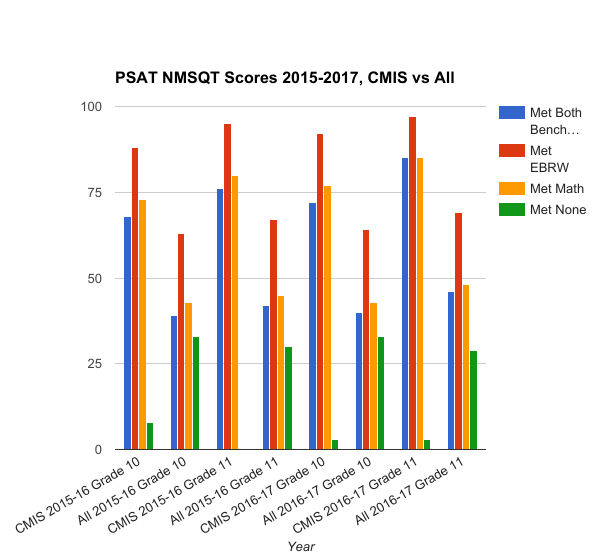
\includegraphics[width=\textwidth]{profile26}
\caption{PSAT NMSQT 2015-2017, CMIS vs All}
\end{figure}

\begin{figure}
\centering
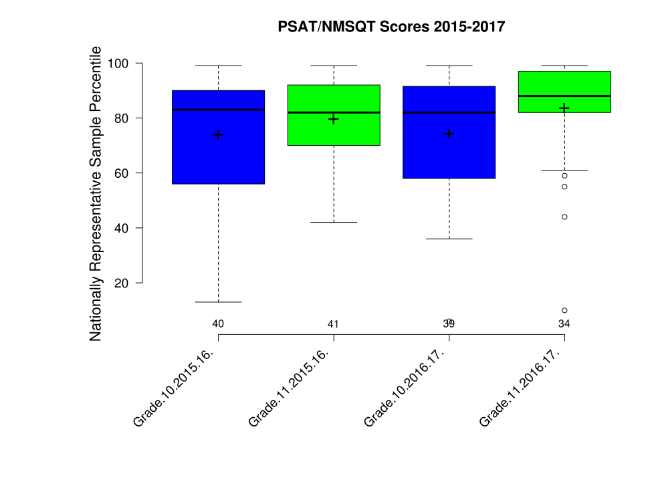
\includegraphics[width=\textwidth]{profile27}
\caption{PSAT/NMSQT Scores 2015-2017}
\end{figure}

\subsection{Scholastic Aptitude Test (SAT)}

CMIS students take the Scholastic Aptitude Test (SAT) in grades 11 and 12.  According to the \href{https://www.prepscholar.com/sat/s/}{prep scholar website} a good score for a college-bound student is at or above 1,000.  An excellent score (top 25\%) falls at or above 1,200.  For the past five years, the average mean score of CMIS SAT-takers has fallen within the range of college-bound students.  (The data from 2015 and earlier has been adjusted using the College Board’s Concordance table.)

\begin{figure}
\centering
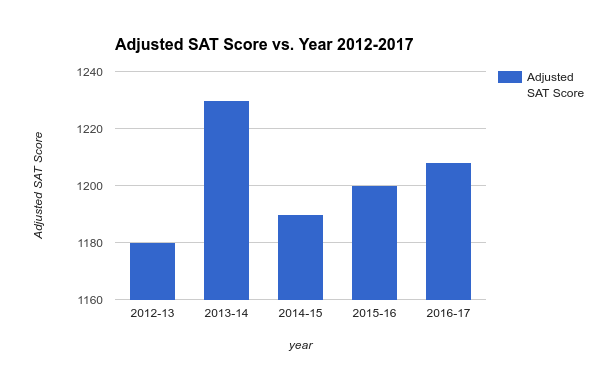
\includegraphics[width=\textwidth]{profile28}
\caption{Adjusted SAT Score vs. Year 2012-2017}
\end{figure}

\subsection{AP Courses}

CMIS has offered a variety of AP course for over 12 years. Students are allowed to enroll in an AP course if they complete the prerequisite courses and obtain teacher approval.  CMIS students who take AP courses historically do very well and score well above the global average, as well the average for international schools in Thailand.  However, CMIS students have the option taking the AP course without taking the AP exam, so many students only choose to take exams for which they feel well prepared.  Over the past 5 years, the AP program at CMIS has increased its course offerings to 19 different courses, and student participation has increased over the past 2 years.

\begin{figure}
\centering
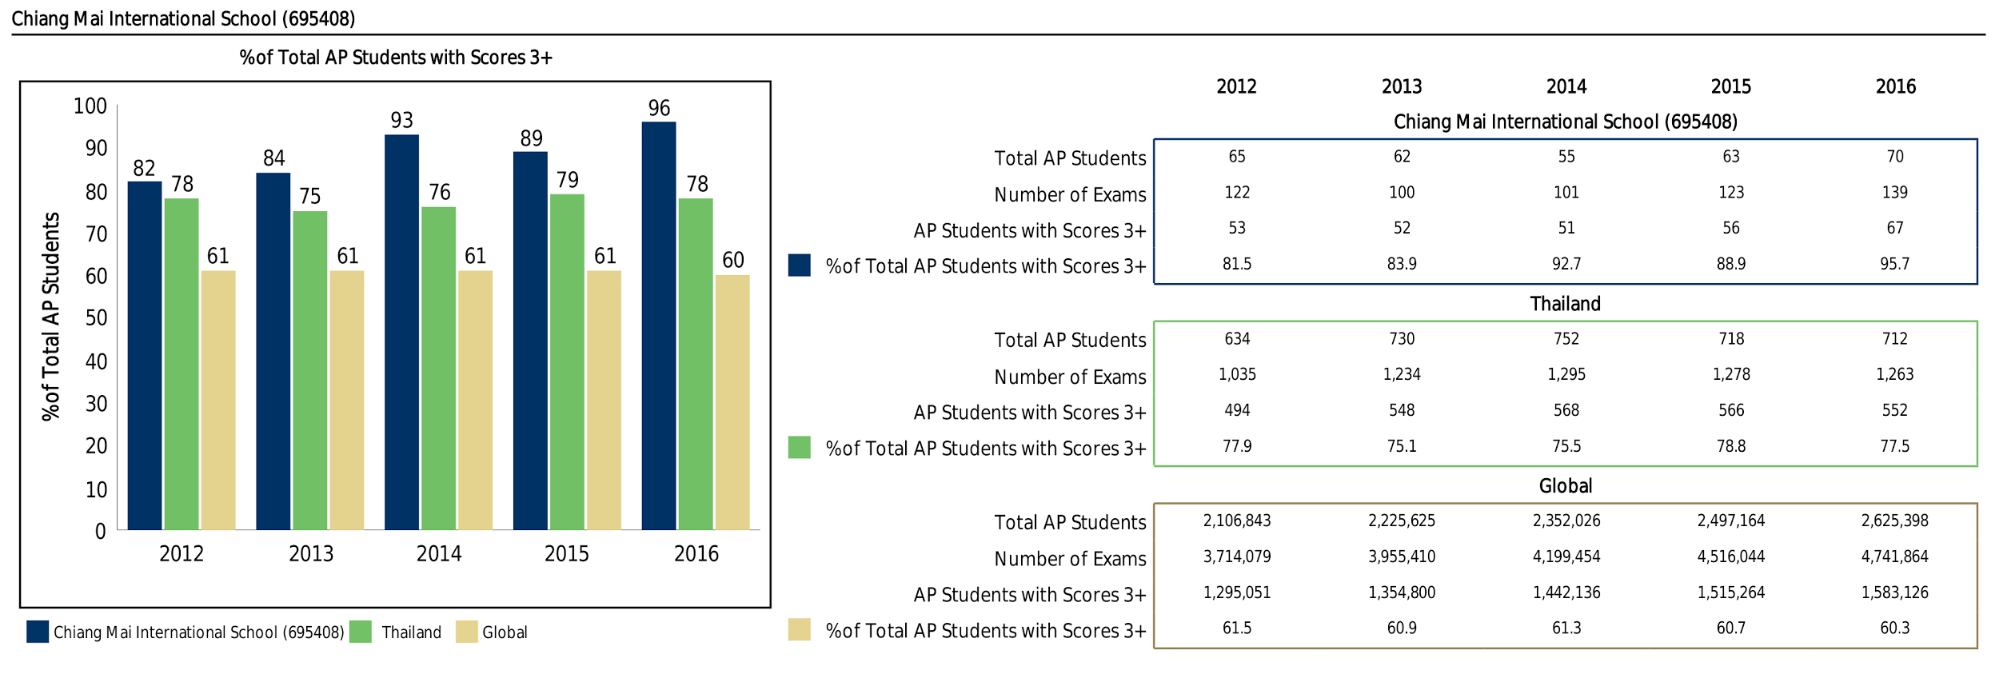
\includegraphics[width=\textwidth]{profile29}
\caption{AP Exam Score Summary}
\end{figure}

\subsection{Students Plans Post Graduation}

College planning for CMIS students begins in Gr. 10.  All Gr. 10 students are required to take the PSAT (Preliminary Scholastic Aptitude Test), and the SAT (Scholastic Aptitude Test) before completion of Gr. 12.  The CMIS College Guidance Counselor works with all eligible students in identifying their options, exploring their possibilities, and planning their applications to colleges and universities.  High school students have been given Overgrad accounts to help track and research interests in careers and universities, mostly in the United States.  

\minor{University Entrance}

\begin{table}
\caption{Post-graduation Plans}
\label{table:13}
\begin{tabu}{|X|X|X|X|X|X|}
\hline
Year &
Number of Seniors &
Enter College/University &
Gap Year &
Did not enter College/University &
\%Matriculating \\
\hline
2015-16 &
37 &
36 &
1 &
0 &
100\% \\
\hline
2014-15 &
36 &
32 &
4 &
0 &
100\% \\
\hline
2013-14 &
40 &
36 &
4 &
0 &
100\% \\
\hline
\end{tabu}
\end{table}

CMIS graduates gain admission to colleges and universities around the world, with many electing to study in North America. Approximately 98\% of CMIS students attend post­-secondary institutions upon graduation. The following is a list of colleges and universities to which CMIS Class of 2015 graduates were offered acceptance.  This information is generally included in our School Profile.

\minor{\href{https://docs.google.com/document/d/1i8tDt8omsO9Zz4Zj40uOpUz8twkbGHYSk_PDs3Rqup4/edit}{Class of 2015-16 College and University Placement}}

In recent years, CMIS graduates have been accepted to a wide variety of international colleges and universities, as listed below. In keeping with this tradition of excellence, students in our 2015 graduating class have been offered acceptance into an impressive array of colleges and universities throughout the world. Those universities in which our current graduates have been offered acceptance are indicated with an asterisk. 

\begin{itemize}
\item Baylor University, Waco, TX
\item *Bentley University, Waltham, MA
\item Boston University, Boston, MA
\item Biola University, La Mirada, CA
\item *Bryn Mawr College, Bryn Mawr, PA
\item *California Polytechnic State University, San Luis Obispo, CA
\item California State University Fullerton, Fullerton, CA
\item *Calvin College, Grand Rapids, MI
\item *Carroll College, Waukesha, WI
\item Clark University, Worcester, MA
\item *Cornell University, Ithaca, NY
\item Davidson College, Davidson, NC
\item Emory University, Atlanta, GA
\item Fordham University, Bronx, NY
\item *Grinnell College, Grinnell, IA
\item *Hult, International Business School, Boston, MA
\item *Ithaca College, New York, NY
\item Lancaster Bible College, Lancaster, PA
\item Lafayette College, Easton, PA
\item Lewis and Clark College, Portland, OR
\item Marquette University, Milwaukee, WI
\item *Messiah College, Mechanicsburg, PA
\item Michigan State University, East Lansing, MI
\item Mississippi State University, MS
\item *Mount Holyoke College, South Hadley, MA
\item *New York University, Greenwich Village, NY
\item *Northeastern University, Boston, MA
\item Ohio Wesleyan University, Delaware, OH
\item Penn State University, State College, PA
\item Purdue University, West Lafayette, IN
\item Rochester Institute of Technology, Rochester, NY
\item Rutgers University, New Brunswick, NJ
\item Rice university, Houston, TX
\item Savannah College of Art and Design (SCAD), Savannah, GA
\item State University of New York, (SUNY), Buffalo, NY
\item Syracuse University, Syracuse, NY
\item Texas A\&M University, College Station, TX
\item *University of Akron, Akron, OH
\item *University of California, Irvine / Davis / Riverside, CA
\item *University of Connecticut, Storrs, CT
\item *University of Illinois Urbana Champaign, Champaign, IL
\item *University of Massachusetts, Amherst, MA
\item *University of Michigan, Ann Arbor, MI
\item University of San Francisco, San Francisco, CA
\item University of Washington, Seattle, WA
\item Vanderbilt University, Nashville, TN
\item Virginia Polytechnic Institute, Blacksburg, VA
\item *Wheaton College, Wheaton, IL
\end{itemize}


Canada:

\begin{itemize}
\item Carleton University, Ottawa, Ontario
\item *Trinity Western University, BC
\item University of British Columbia, Vancouver, BC
\item * University of Toronto
\item *University of Waterloo, Toronto
\end{itemize}


Europe:

\begin{itemize}
\item *Ecole hoteliere de Lausanne, Lausanne, Switzerland
\item *Eindhoven University of Technology, Netherlands
\item Erasmus University College, Rotterdam, Netherlands
\item *Hague University of Applied Science, Netherlands
\item *Hanze University, Groningen, Netherlands
\item University College Roosevelt, Middelburg, Zeeland, Netherlands
\item University of Groningen (RUG), Groningen, Netherlands
\item *University of Aberdeen, Scotland, UK
\item *University of Nottingham, England, UK
\item *University of Sheffield, England, UK
\item *University of Stirling, Scotland, UK
\item *University of Strathclyde, Scotland, UK
\end{itemize}

Australia:

\begin{itemize}
\item *Le Cordon Bleu, Culinary Arts Institute, Sydney
\item *Blue Mountains, International Hotel Management School, Sydney
\end{itemize}


Thailand:

\begin{itemize}
\item *Assumption, University, (ABAC), Bangkok
\item *Chulalongkorn University, Bangkok
\item *Mahidol University, Bangkok
\item Payap University, Chiang Mai
\item *Thammasat University, Bangkok
\end{itemize}


Other Parts of Asia:

\begin{itemize}
\item *Ritsumeikan Asia Pacific University, Oita, Japan
\item *Nanyang Technological University, Singapore
\item *Shanghai Jiao Tong University, Shanghai, China
\item *State University of New York (SUNY), Seoul, Korea
\end{itemize}


\tcbsection{School Community Surveys (Teacher, Student, Community}

Every academic year, in May, CMIS sends out opinion surveys to the community.  Results from the surveys provide data regarding community perception in the areas of curriculum, learning, and school environment. 

The demographic groups surveyed are: teachers and staff, students grade 4-12, and CMIS Families. The questions in each survey are targeted to the corresponding demographic group. In order to capture data from our entire community, the CMIS Family survey is provided in English, Korean, and Thai (the three major segments of the student/family population).

Administration review the survey data and use responses to guide planning and target areas for improvement.

\subsection{Teacher Survey}

At the beginning of the 2016-17 school year the Administrative Team (principals and superintendent) analyzed the 2015-16 CMIS staff survey together and identified two items for improvement:
\begin{itemize}
\item My administrator knows what is going on in my classroom.
\item If I am feeling stressed out or overloaded, I feel comfortable talking to my division administrator. 
\end{itemize}


During the September professional development early dismissal day, the administrative team shared the areas with the staff and asked for anonymous suggestions of ways to improve. From these suggestions came the following three initiatives:
\begin{itemize}
\item A weekly schedule of classroom walkthroughs by principals, PK-12.  The schedule provides consistency and helps address the the issue of “My administrator knows what is going on in my classroom”.
\item Principals and Superintendent visible and available on the playground every day before school starts.  This opportunity provides a personal opportunity for staff to easily locate and approach the administrative team.
\item Department Check-Ins completed by the Superintendent (via-email or during Team Leader meetings), where team leaders are asked to identify the needs of their team and encouraged to share ideas of how the Administrative Team can best support them.
\end{itemize}

The Administrative Team will complete a brief staff survey in February as a way to assess perceptions of the above initiatives.  A Summary of CMIS Staff Survey \ref{table:14} results is included below.   


\begin{figure}
\centering
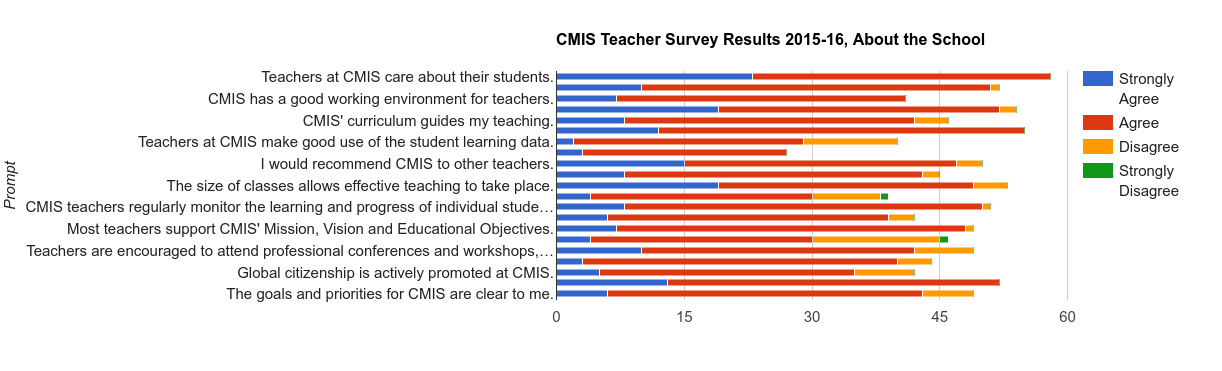
\includegraphics[width=\textwidth]{profile30}
\caption{CMIS Teacher Survey Results 2015-2016, About the School}
\end{figure}

\begin{figure}
\centering
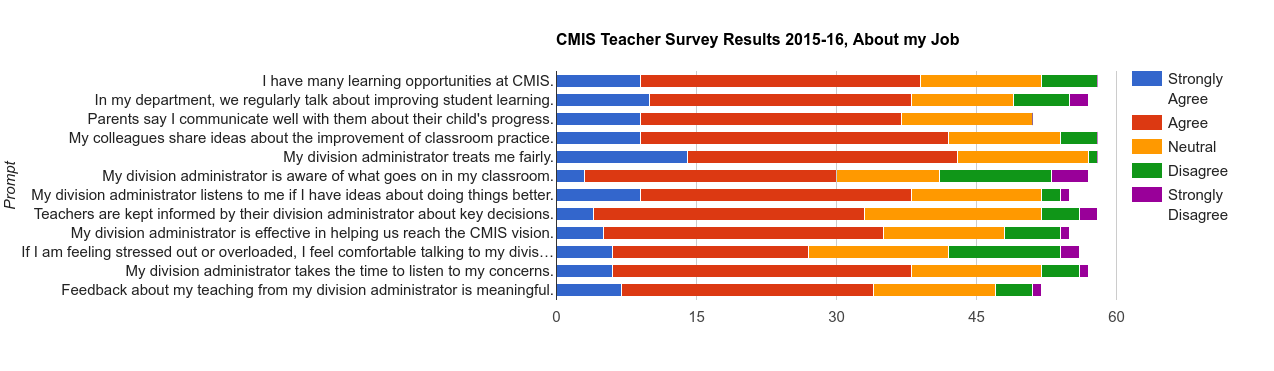
\includegraphics[width=\textwidth]{profile31}
\caption{CMIS Teacher Survey Results 2015-2016, About my Job}
\end{figure}

\begin{figure}
\centering
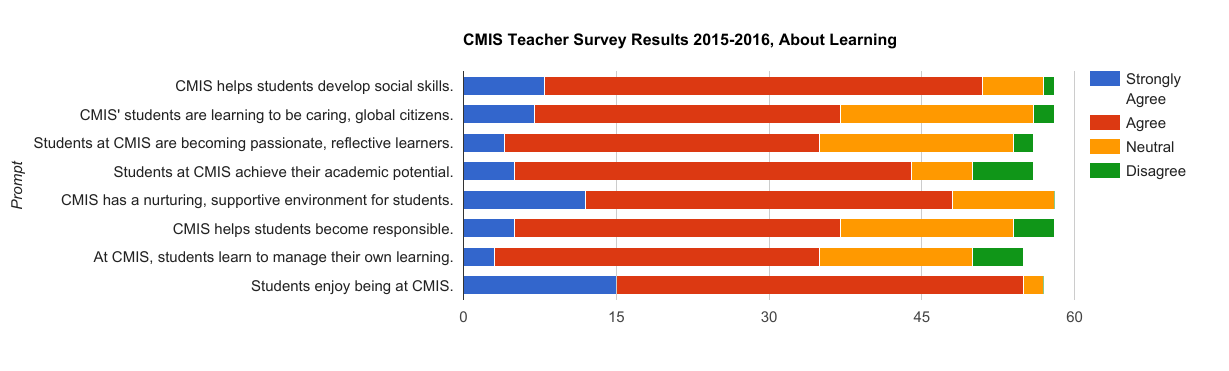
\includegraphics[width=\textwidth]{profile32}
\caption{CMIS Teacher Survey Results, About Learning}
\end{figure}

\subsection{Family Survey}

During the 2016 Board retreat, the Board analyzed the\href{https://docs.google.com/a/cmis.ac.th/forms/d/16Gbd3MzQOXtjjZ2dG460xw5SHG_eohMIKet3lxYUdAY/edit#responses}{ 2015-16 CMIS Family Survey} and identified two areas for improvement:
\begin{itemize}
\item Communication
\item Who does what, roles of the CMIS board members
\end{itemize}


These items are addressed by the following initiatives:
\begin{itemize}
\item Creating a forum where the \href{https://docs.google.com/document/d/1kiwakkg8eKdtEexCxVNx-m1CfC3VqxhukDy8WXDPGKY/edit?ts=58a2a142}{community determines what is presented} during the PTG meetings. Instead of the school driving the content presented to the community during these meetings, PTG meetings are driven by what the community wants. For example, topics such as college and career counseling, technology use, student activities, student health with regard to Chiang Mai’s burning season, etc. have been recent topics identified by the community and discussed at PTG meetings.
\item What’s happening with the board? - CMIS board meeting summaries are created and posted on the CMIS PTG website, allowing more access and transparency to what is being discussed at the board level.
\item Who does what? - at least four CMIS board members attend every PTG meeting, these members are identified so that parents have a greater sense of who is on the CMIS board. CMIS board members attend and speak at CMIS events whenever possible, for example, back-to-school bbq, CMIS Christmas Concert, CMIS Plays, CMIS Latin Night, etc. Additionally, CMIS board members, the roles and responsibilities of the board and it’s individual members will be displayed on the CMIS website.
\end{itemize}

The Board will follow up with a community, “Sounding Board” session in March 2017 as an informal way to assess perceptions of the above initiatives.  A \href{https://docs.google.com/a/cmis.ac.th/document/d/1_otvw47y3Z-1CSjXnKhgRTauVRqPl1S6nSdmsb00O2k/edit?usp=sharing}{summary of the CMIS Family Survey} results is included in table \ref{table:14}:  

\begin{table}[h]
\tiny
\caption{Family Survey of Board/Leadership}
\label{table:14}
\tabulinesep=^2pt_2pt
\begin{longtabu}{|X[8]|X|X|}
\hline
Family Survey Questions related to Board/Leadership out of 127 responses &
\#/127 Agree &
\#/127 Disagree \\
\hline
The Board provides good representation for the CMIS community &
60 &
17 (13\%) \\
\hline
The Board makes decisions that help CMIS and plan for the future &
66 &
10 \\
\hline
The Board and school leadership execute responsible resource planning for the future &
61 &
16 (13\%) \\
\hline
The Board encourages suggestions and feedback about improving CMIS &
62 &
19 (15\%) \\
\hline
The Board works actively to improve CMIS &
64 &
14 (11\%) \\
\hline
The Board models the qualities of respect, fairness, equity, integrity, and honesty in professional dealings with others. &
62 &
10 \\
\hline
The Board communicates effectively with the CMIS community &
57 &
21 (17\%) \\
\hline
The Board respects diversity, valuing people and cultures represented in the school and by the community at large. &
71 &
8 \\
\hline
The Director makes decisions that help CMIS and plan for the future &
61 &
5 \\
\hline
The Director and school leadership execute responsible resource planning for the future &
59 &
9 \\
\hline
The Director encourages suggestions and feedback about improving CMIS &
54 &
17 (13\%) \\
\hline
The Director works actively to improve CMIS &
59 &
8 \\
\hline
The Director communicates effectively with the CMIS community &
54 &
19 (15\%) \\
\hline
The Director models the qualities of respect, fairness, equity, integrity, and honesty in professional dealings with others. &
60 &
7 \\
\hline
The Director respects diversity, valuing people and cultures represented in the school and by the community at large. &
60 &
4 \\
\hline
The Manager makes decisions that help CMIS and plan for the future &
65 &
6 \\
\hline
The Manager and school leadership execute responsible resource planning for the future &
58 &
10 \\
\hline
The Manager encourages suggestions and feedback about improving CMIS &
59 &
12 \\
\hline
The Manager works actively to improve CMIS &
62 &
5 \\
\hline
The Manager communicates effectively with the CMIS community &
65 &
12 \\
\hline
The Manager models the qualities of respect, fairness, equity, integrity, and honesty in professional dealings with others. &
60 &
3 \\
\hline
The Manager respects diversity, valuing people and cultures represented in the school and by the community at large. &
61 &
3 \\
\hline
The Superintendent makes decisions that help CMIS and plan for the future &
77 &
4 \\
\hline
The Superintendent and school leadership execute responsible resource planning for the future &
75 &
5 \\
\hline
The Superintendent encourages suggestions and feedback about improving CMIS &
71 &
10 \\
\hline
The Superintendent works actively to improve CMIS &
75 &
4 \\
\hline
The Superintendent provides effective leadership for student achievement &
67 &
4 \\
\hline
The Superintendent provides effective leadership for appropriate student behaviour &
66 &
7 \\
\hline
The Superintendent provides effective leadership for teacher supervision (hiring, evaluation, etc.) &
64 &
8 \\
\hline
The Superintendent communicates effectively with the CMIS community &
73 &
7 \\
\hline
The Superintendent models the qualities of respect, fairness, equity, integrity, and honesty in professional dealings with others. &
72 &
2 \\
\hline
The Superintendent respects diversity, valuing people and cultures represented in the school and by the community at large. &
76 &
2 \\
\hline
The HS Principal provides effective leadership for student achievement &
39 &
3 \\
\hline
The HS Principal provides effective leadership for appropriate student behaviour &
38 &
7 \\
\hline
The HS Principal makes decisions that help CMIS and plan for the future &
41 &
3 \\
\hline
The HS Principal encourages suggestions and feedback about improving CMIS &
40 &
2 \\
\hline
The HS Principal works actively to improve CMIS &
40 &
2 \\
\hline
The HS Principal communicates effectively with the CMIS community &
41 &
2 \\
\hline
The HS Principal models the qualities of respect, fairness, equity, integrity, and honesty in professional dealings with others. &
40 &
4 \\
\hline
The HS Principal respects diversity, valuing people and cultures represented in the school and by the community at large. &
31 &
1 \\
\hline
The MS Principal provides effective leadership for student achievement &
45 &
4 \\
\hline
The MS Principal provides effective leadership for appropriate student behaviour &
46 &
2 \\
\hline
The MS Principal makes decisions that help CMIS and plan for the future &
44 &
3 \\
\hline
The MS Principal encourages suggestions and feedback about improving CMIS &
41 &
8 \\
\hline
The MS Principal works actively to improve CMIS &
46 &
4 \\
\hline
The MS Principal communicates effectively with the CMIS community &
43 &
6 \\
\hline
The MS Principal models the qualities of respect, fairness, equity, integrity, and honesty in professional dealings with others. &
44 &
4 \\
\hline
The MS Principal respects diversity, valuing people and cultures represented in the school and by the community at large. &
47 &
3 \\
\hline
The Elementary Principal makes decisions that help CMIS and plan for the future &
50 &
2 \\
\hline
The Elementary Principal encourages suggestions and feedback about improving CMIS &
49 &
5 \\
\hline
The Elementary Principal provides effective leadership for appropriate student behaviour &
52 &
4 \\
\hline
The Elementary Principal provides effective leadership for student achievement &
49 &
3 \\
\hline
The Elementary Principal works actively to improve CMIS &
50 &
3 \\
\hline
The Elementary Principal communicates effectively with the CMIS community &
48 &
5 \\
\hline
The Elementary Principal models the qualities of respect, fairness, equity, integrity, and honesty in professional dealings with others. &
49 &
4 \\
\hline
The Elementary Principal respects diversity, valuing people and cultures represented in the school and by the community at large. &
50 &
4 \\
\hline
\end{longtabu}
* Bolded items have more than a 10\% score of DISAGREE

English = 77 respondents
Thai = 39 respondents
Korean = 11 respondents
Total respondents = 127

Surveyed families represent the following students: 
ES respondents (children in PreK to G4) = 54
Grade 5 and MS (children in G5 to G8) = 68
HS respondents (children in G9 to G12) = 44
\end{table}


\subsection{\href{https://docs.google.com/a/cmis.ac.th/forms/d/1n7vFCQbPQmF6pEPJKPBsu4rzdiW4KQ_DrBcjTMUbLH4/viewanalytics}{Student Survey}}

In May 2016, students in grades 4 through 12 were given a student survey to gather perceptions on CMIS as a whole, their teachers, and their learning.  Below are the results of the 2015-2016 Student Survey.  

\begin{figure}
\centering
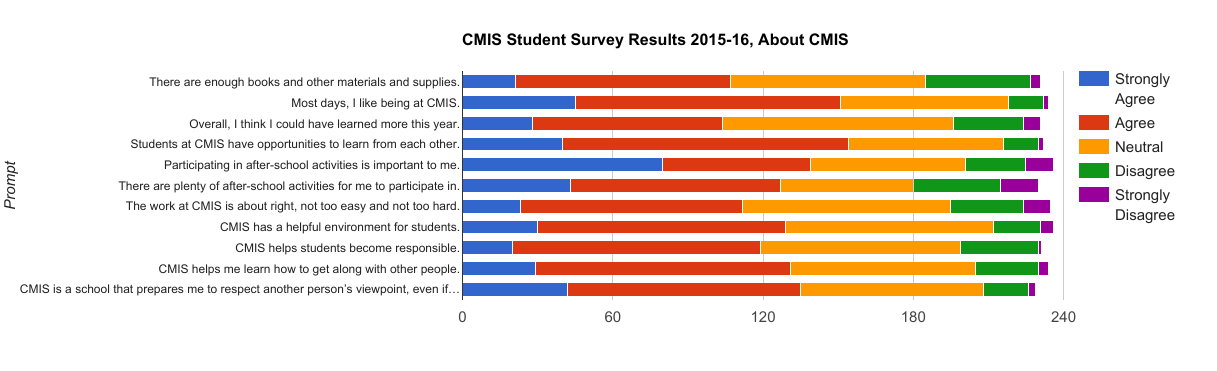
\includegraphics[width=\textwidth]{profile33}
\caption{CMIS Student Survey Results 2015-2016, About CMIS}
\end{figure}

\begin{figure}
\centering
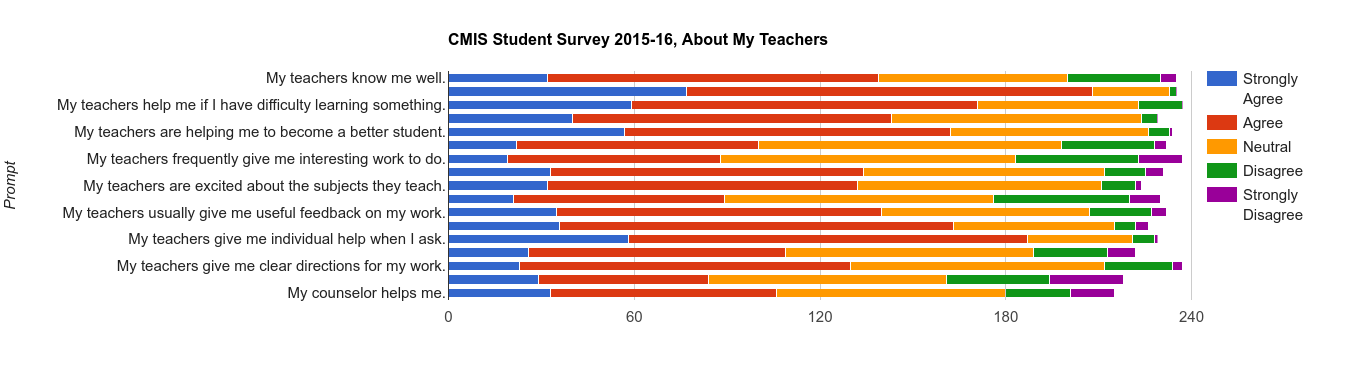
\includegraphics[width=\textwidth]{profile34}
\caption{CMIS Student Survey Results 2015-2016, About My Teachers}
\end{figure}

\begin{figure}
\centering
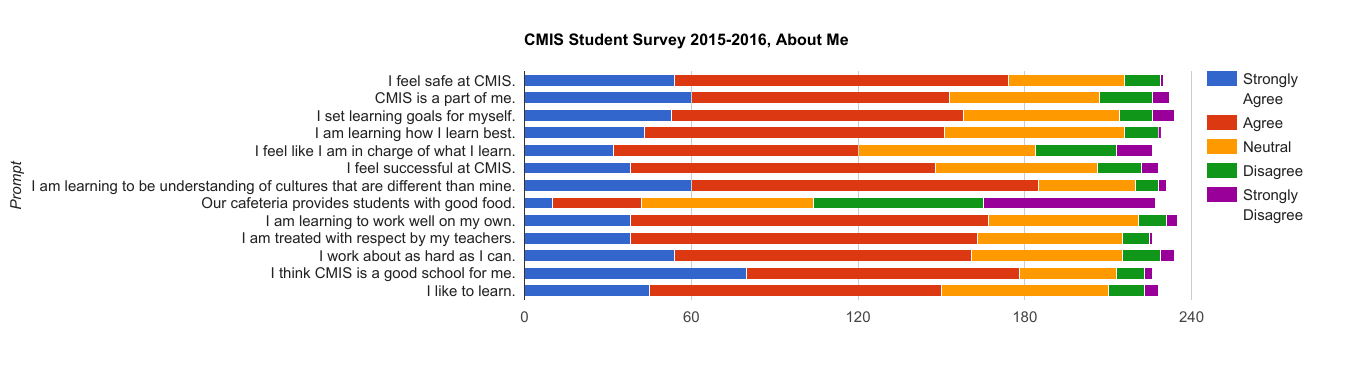
\includegraphics[width=\textwidth]{profile35}
\caption{CMIS Student Survey Results 2015-2016, About Me}
\end{figure}

At the beginning of the 2016-17 school year the SET (director, manager, superintendent) analyzed the 2015-16 CMIS Student Survey and identified two areas for improvement:
\begin{itemize}
\item School Cafeteria - food quality, price, and variety
\item Availability of student activities
\end{itemize}

\begin{figure}
\centering
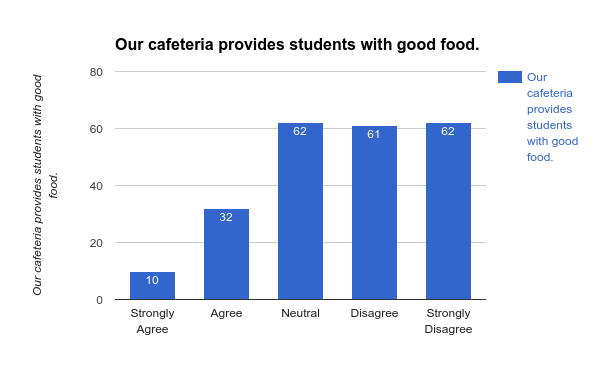
\includegraphics[width=\textwidth]{profile36}
\caption{Cafeteria Survey Results}
\end{figure}

\minor{Follow Up Cafeteria Survey}

To address the School Cafeteria concerns, a \href{https://docs.google.com/a/cmis.ac.th/forms/d/18wFe46SOpPVv9_jkKLEa4OqVsDkLtJkUCcM85Jul0Ik/viewanalytics}{survey} was constructed by the Health Officer and sent to all students. The purpose of the survey was to further identify issues existing with the school cafeteria. Actionable items resulting from the survey were: 

\begin{itemize}
\item Price 
\item Cafeteria lines
\item Availability of food (especially for MS/HS students)l
\item Variety of food available (especially for MS/HS students) 
\item Cafeteria design/size/temperature
\end{itemize}


The SET created a cafeteria committee who met with the contractors to discuss possible resolutions. As a result of this meeting:
\begin{itemize}
\item An increased variety of food is being offered
\item Snacks and pre made food  have been moved out of the cafeteria to improve the flow and shorten lines
\item Plans to expand the outdoor dining area and are now underway
\item Changes have been made to the new cafeteria building plans to address suggestions that came out of the survey 
\end{itemize}

The cafeteria committee will follow up with an additional survey to measure student perceptions of the above changes.

With regard to availability of student activities, an elementary activity coordinator position was created (additional assignment to an existing teacher).  The elementary activity coordinator is in charge of organizing all elementary activities and clubs, checking to ensure that there is a wide variety of activities (something for everyone), and maintaining a central location for all information about elementary activities and clubs.

\subsection{New Family Survey}

Newly admitted students’ families are given a \href{https://docs.google.com/a/cmis.ac.th/forms/d/1basukpCBjcCMWXDh-cUUWW6lgk6zxYadGMn1EzFDQwc/viewanalytics}{New Family Survey} to help identify areas on which we need to focus; both in terms of the student application process and advertising. We use this data to refine how we reach our target audience and provide a better experience for our new families.

\begin{figure}
\centering
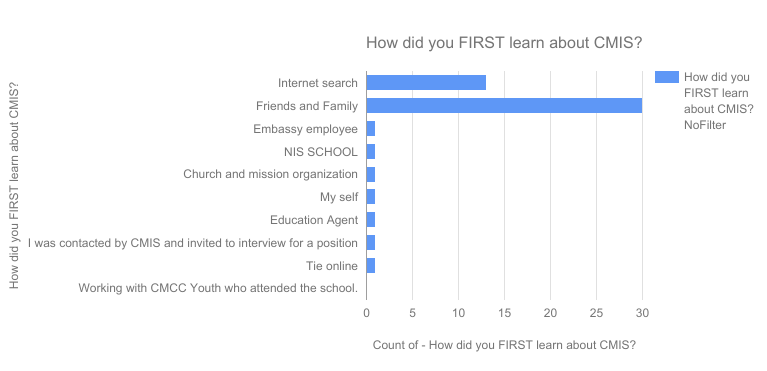
\includegraphics[width=\textwidth]{profile37}
\caption{How did you FIRST learn about CMIS?}
\end{figure}

Results of the New Family Survey show that most of our new families learn about CMIS from word-of-mouth, followed by Internet search. Knowing this has enabled us to focus our attention on these two areas of publicizing the school. In the 2016-17 academic year a new version of the school website was launched. Emphasis was put on highlighting the best parts of CMIS and making it easy for new families to find information about admission, enrollment, and student life.

\begin{figure}
\centering
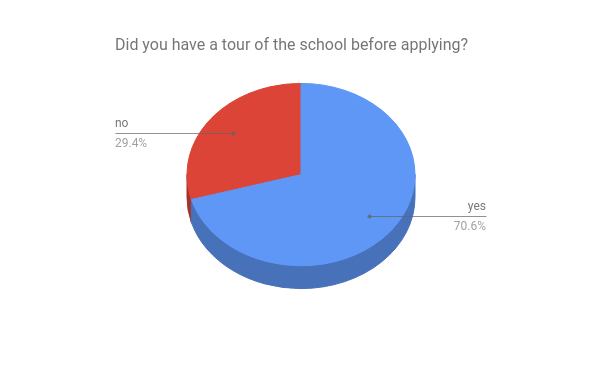
\includegraphics[width=\textwidth]{profile38}
\caption{Tour Survey Question 1}
\end{figure}

\begin{figure}
\centering
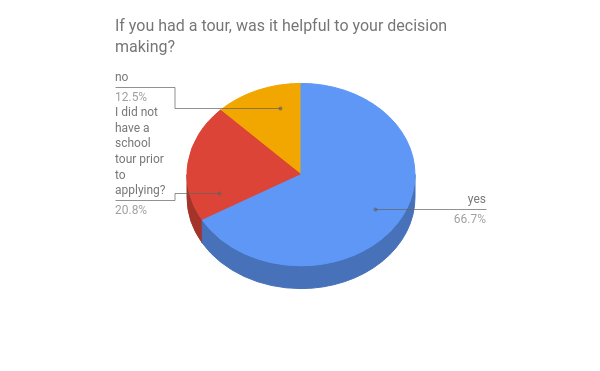
\includegraphics[width=\textwidth]{profile39}
\caption{Tour Survey Questions 2}
\end{figure}

\begin{figure}
\centering
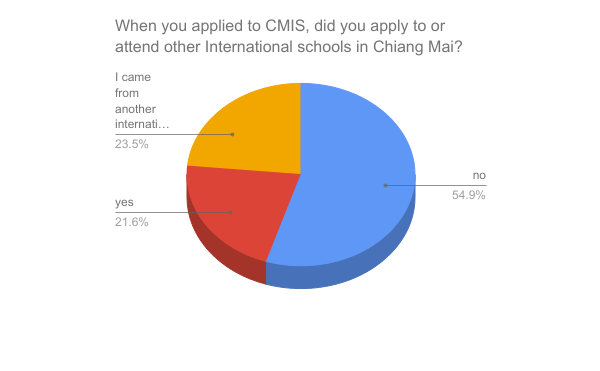
\includegraphics[width=\textwidth]{profile40}
\caption{Tour Survey Question 3}
\end{figure}

We also learned that most respondents had a school tour prior to applying, 70\%, and that the school tour was helpful in making the decision, 66\%. Additionally families surveyed did not apply to other international schools in Chiang Mai, indicating CMIS as their school of choice.

Of the reasons Families choose CMIS, Teachers, Community, and Curriculum were the most prevalent followed by the diversity of the student population, facilities, and location. Tuition was not indicated as a factor in deciding to come to CMIS.

\tcbsection{Conclusion}

Since our last WASC report in 2011, CMIS has gone through a period of growth and development, while remaining true to its mission and vision. Enrollment and staffing have increased incrementally, and a plan has been implemented to develop the facilities accordingly. Our Board and school leadership teams have held firmly to our school mission and vision by developing and refining our Student Learner Outcomes. 

Increased demand for enrollment has presented us with opportunities to maximize student diversity and apply higher standards for entry. We maintain a diverse student population, and select qualified, priority applicants for enrollment before considering all others on a space-available basis. We also place limits on our population's demographics in order to maintain the school's English-speaking environment and diverse, international character. 
 
Application to CMIS is competitive, and managed through an online application system. Newly selected students are surveyed to help identify areas in which we need to improve our processes and focus our advertising. The respective roles of the school website and the admissions tour have been identified as important factors affecting our applicants' decision to apply to CMIS. 

All students have to demonstrate English-language proficiency and qualify academically for their grade level before they can be considered for enrollment. Students are also required to meet the behavioral, emotional, and social expectations of the CMIS student body. Applicants are selected by an Admissions Committee, who also considers the available resources and existing student population when selecting new students.  

The quality of our teaching staff ranks highly among the reasons why people choose to study at CMIS. Our teachers are highly qualified, and our school's administrative structure is effective for efficient operation and management. CMIS has demonstrated its commitment to obtaining and retaining quality teaching staff by providing increased opportunities for Professional Development (PD). Since the time of our last WASC report, monthly scheduled PD time as well as a designated fund for professional development has been established and utilized to effectively support student learning through teacher training.

Our teachers and administrators are satisfied with the working conditions at CMIS, and often stay for multiple 2-year contract periods. The diversity of our teaching staff provides a stimulating environment in which our cultural differences are celebrated and respected. We currently have staff from 15 different countries. All staff are required to be fully certified and have at least a Bachelor's degree in their respective areas of expertise. Over a third of our staff possess advanced degrees.

College planning is an integral part of our CMIS high school program. Our students are given guidance and assistance in planning their applications for admission to colleges and universities around the world. In general, all of our graduating seniors are matriculated into the programs of their choice, with some choosing to take a gap year to perform community service before beginning their post-secondary studies. 

Opinion surveys have been used to solicit feedback from students, staff, and members of our CMIS community. Responses to surveys have helped guide our school administrators in targeting improvements for each respective group. Whenever areas of concern have been identified, actions have been taken to address the situation and progress has been communicated to the affected community. School administrators have continued to encourage communication through various venues, including staff meetings, student communication groups, monthly PTG meetings, and the Teacher/Administration Communication Team (TACT). 

An emphasis on research-based management led to the realization that limited data was available on CMIS Student Learner Outcomes. The Datawise initiative was taken in response to the need for qualitative data on student performance. Steps were taken to understand the available DRAs, PSAT and SAT scores, AP test results, and ISA test results in light of the CMIS Common Core Objectives. To the extent possible, this data was used to identify student needs and create action plans for improvement. In addition, CMIS has adopted the NWEA MAP (Measures of Academic Progress) school wide in order to produce more useful data that can be used to support modifying student instruction.  

CMIS places high importance on providing opportunities for Student Life Beyond the Classroom. Much has been done to identify and address items of concern to our CMIS community. We will continue the process of annually refining and conducting perception surveys. As a school, we regularly celebrate the progress we are making and make concerted efforts to share this information throughout the CMIS community. 

We are blessed with an intelligent, talented, caring, group of highly qualified staff. Our administrative structure is supportive of staff and schoolwide initiatives. Leadership is effective in implementing change and responding to the needs of our community. The result has been a greater focus on student learning and closer adherence to our school mission and vision. 

The process of looking at data has identified the need for additional data, especially with respect to student learning and performance, and the need for a central data repository. The school will continue to involve all stakeholders in the improvement process, knowing that a collaborative, consultative approach to planning and implementation is the most effective means to bring about and sustain positive, long-lasting change that promotes student learning. 
